\section{Retrieval Augmented Generation} % (fold)
\label{sec:rag}
%
\begin{frame}[t] \frametitle{\emph{Retrieval Augmented Generation}}
\framesubtitle{Criticità simple/stuff prompting}
{\footnotesize
\onslide<1->
    \begin{minipage}[t]{\textwidth}
        \begin{itemize}[leftmargin=10pt,align=right]
            \onslide<1->\item[\alert{\faArrowCircleRight}] \alert{\textit{Simple prompting}}: utente costruisce il contesto manualmente
            \begin{itemize}[leftmargin=10pt,align=right]
                \onslide<2->\item[\alert{\faExclamationTriangle}] LLM genera una risposta in base alla conoscenza su cui è stato addestrato (\alert{\textit{knowledge cut-off}})
                \onslide<3->\item[\alert{\faExclamationTriangle}] Impensabile pre-addestrare LLM su quanlunque sotto-dominio specifico
                \onslide<4->\item[\alert{\faExclamationTriangle}] Quando informazione contestuale non è sufficiente, LLM tende a generare risposte non veritiere (\alert{\textit{hallucination}})
            \end{itemize}
            \onslide<5->\item[\alert{\faArrowCircleRight}] \alert{\textit{Prompt stuffing}}: contesto utente arricchito dinamicamente (es. \textit{chat memory}) 
            \begin{itemize}[leftmargin=10pt,align=right]
                \onslide<6->\item[\alert{\faExclamationTriangle}] \textit{Prompt} potenzialmente eccessivi in grandezza
                \onslide<7->\item[\alert{\faExclamationTriangle}] Problematiche di \textit{context window}
                \onslide<8->\item[\alert{\faExclamationTriangle}] Costi esorbitanti con LLM commerciali
                \onslide<9->\item[\alert{\faExclamationTriangle}] Tempi di risposta proibitivi con LLM \textit{open source}
            \end{itemize}
        \end{itemize}
    \end{minipage}
}
\end{frame}
%
\begin{frame}[t] \frametitle{\emph{Retrieval Augmented Generation}}
\framesubtitle{Natura dinamica dei contenuti digitali}
\vspace*{-.5cm}
{\scriptsize
\onslide<1->
    \begin{minipage}[t]{\textwidth}
        \begin{figure}
            \centering
            
\includegraphics[width=.25\textwidth]{img/RAG_1-scaled.PNG}
            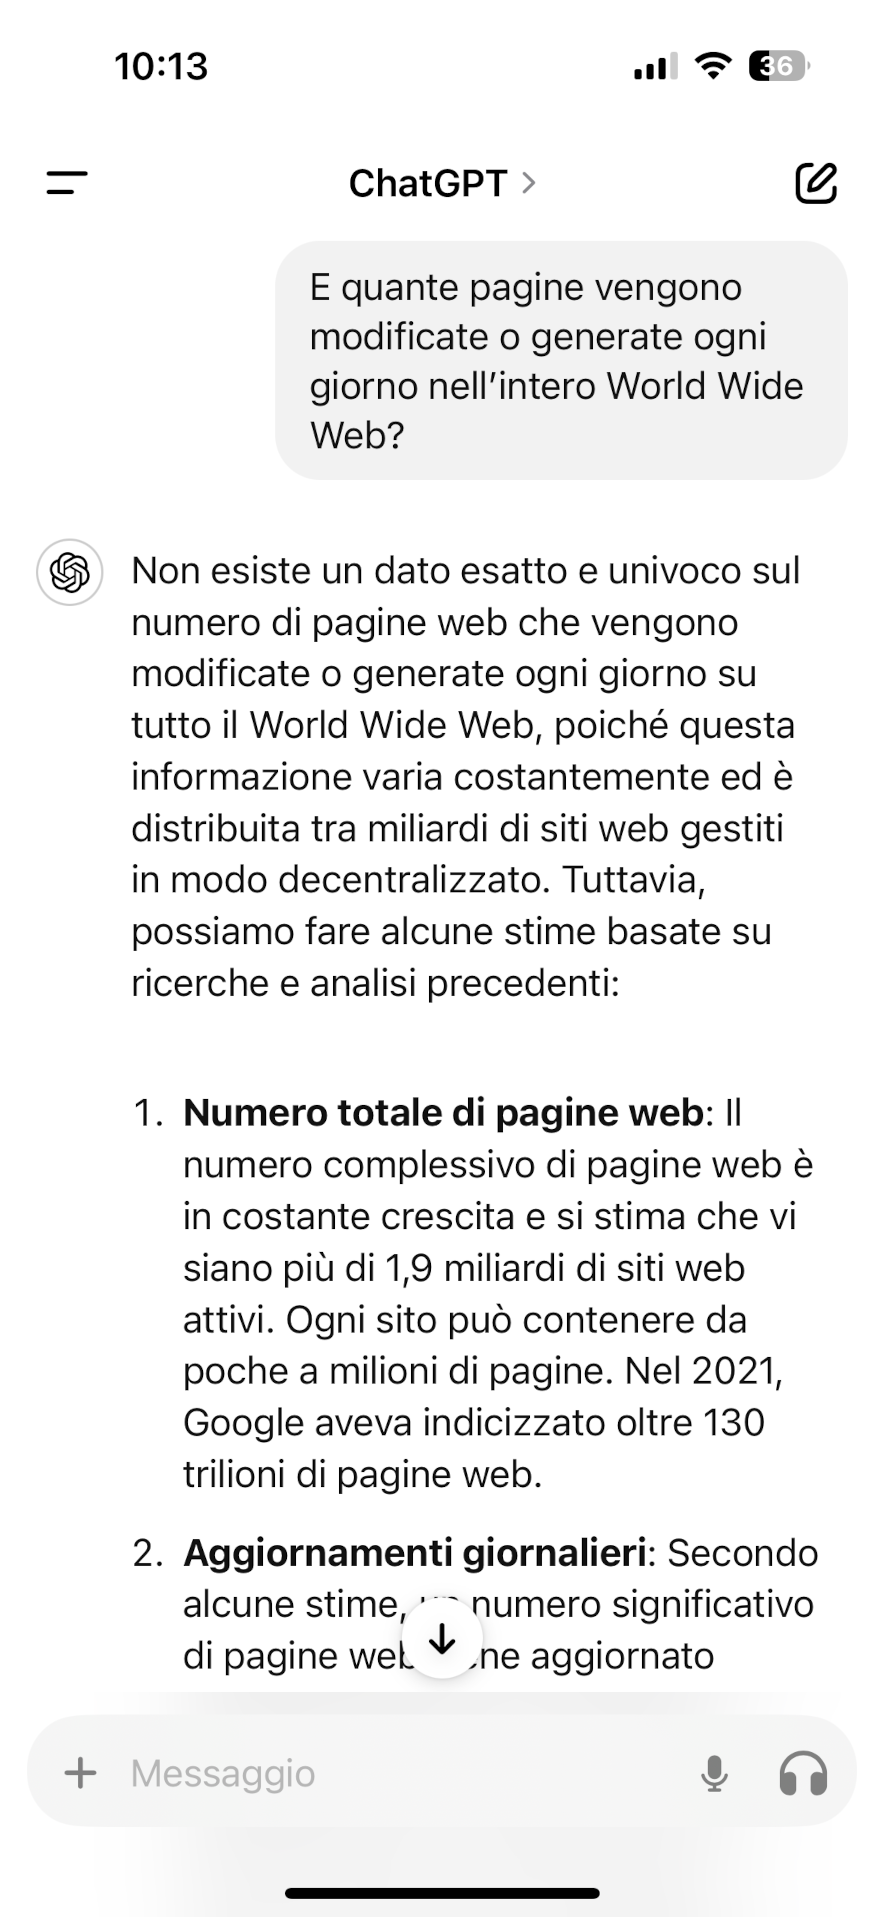
\includegraphics[width=.25\textwidth]{img/RAG_2-scaled.PNG}
            $\cdots$
            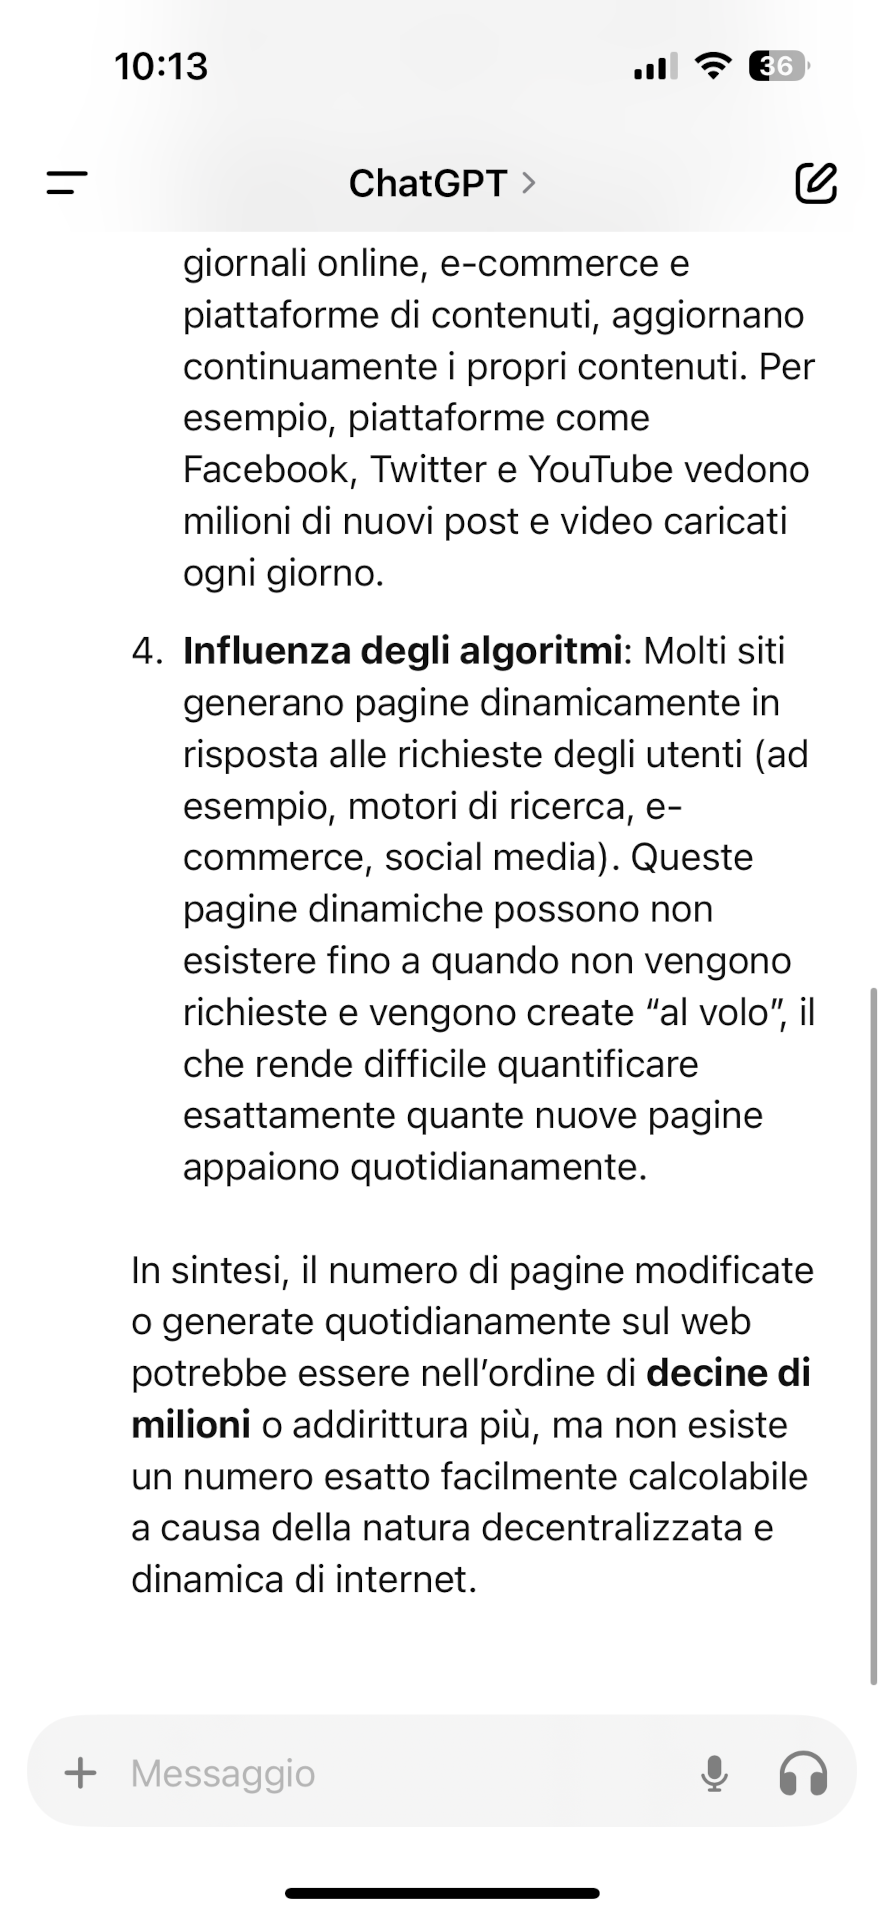
\includegraphics[width=.25\textwidth]{img/RAG_4-scaled.PNG}
        \end{figure}
    \end{minipage}
    \begin{minipage}[t]{\textwidth}
        \vspace*{.3cm}
        \begin{itemize}[leftmargin=10pt,align=right]
            \onslide<2->\item[\alert{\faArrowCircleRight}] Pre-addestramento costante per le LLM non è efficiente
            \onslide<3->\item[\alert{\faArrowCircleRight}] Come fare con \alert{fattoidi} (es. cariche politiche, popolazione per stato, $\ldots$)?!
        \end{itemize}
    \end{minipage}
}
\end{frame}
%
\begin{frame}[t] \frametitle{\emph{Retrieval Augmented Generation}}
{\scriptsize
\onslide<1->
\framesubtitle{Rivoluzione nel mondo dell'addestramento LLM}
\vspace*{-.5cm}
    \begin{minipage}[t]{\textwidth}
        \begin{figure}[ht]
            \centering
            \includegraphics[width=\textwidth]{img/AI-timeline-2021-2.png}
        \end{figure}
    \end{minipage}
    \onslide<1->
    \begin{minipage}[t]{.60\textwidth}
        \begin{figure}[ht]
            \centering
            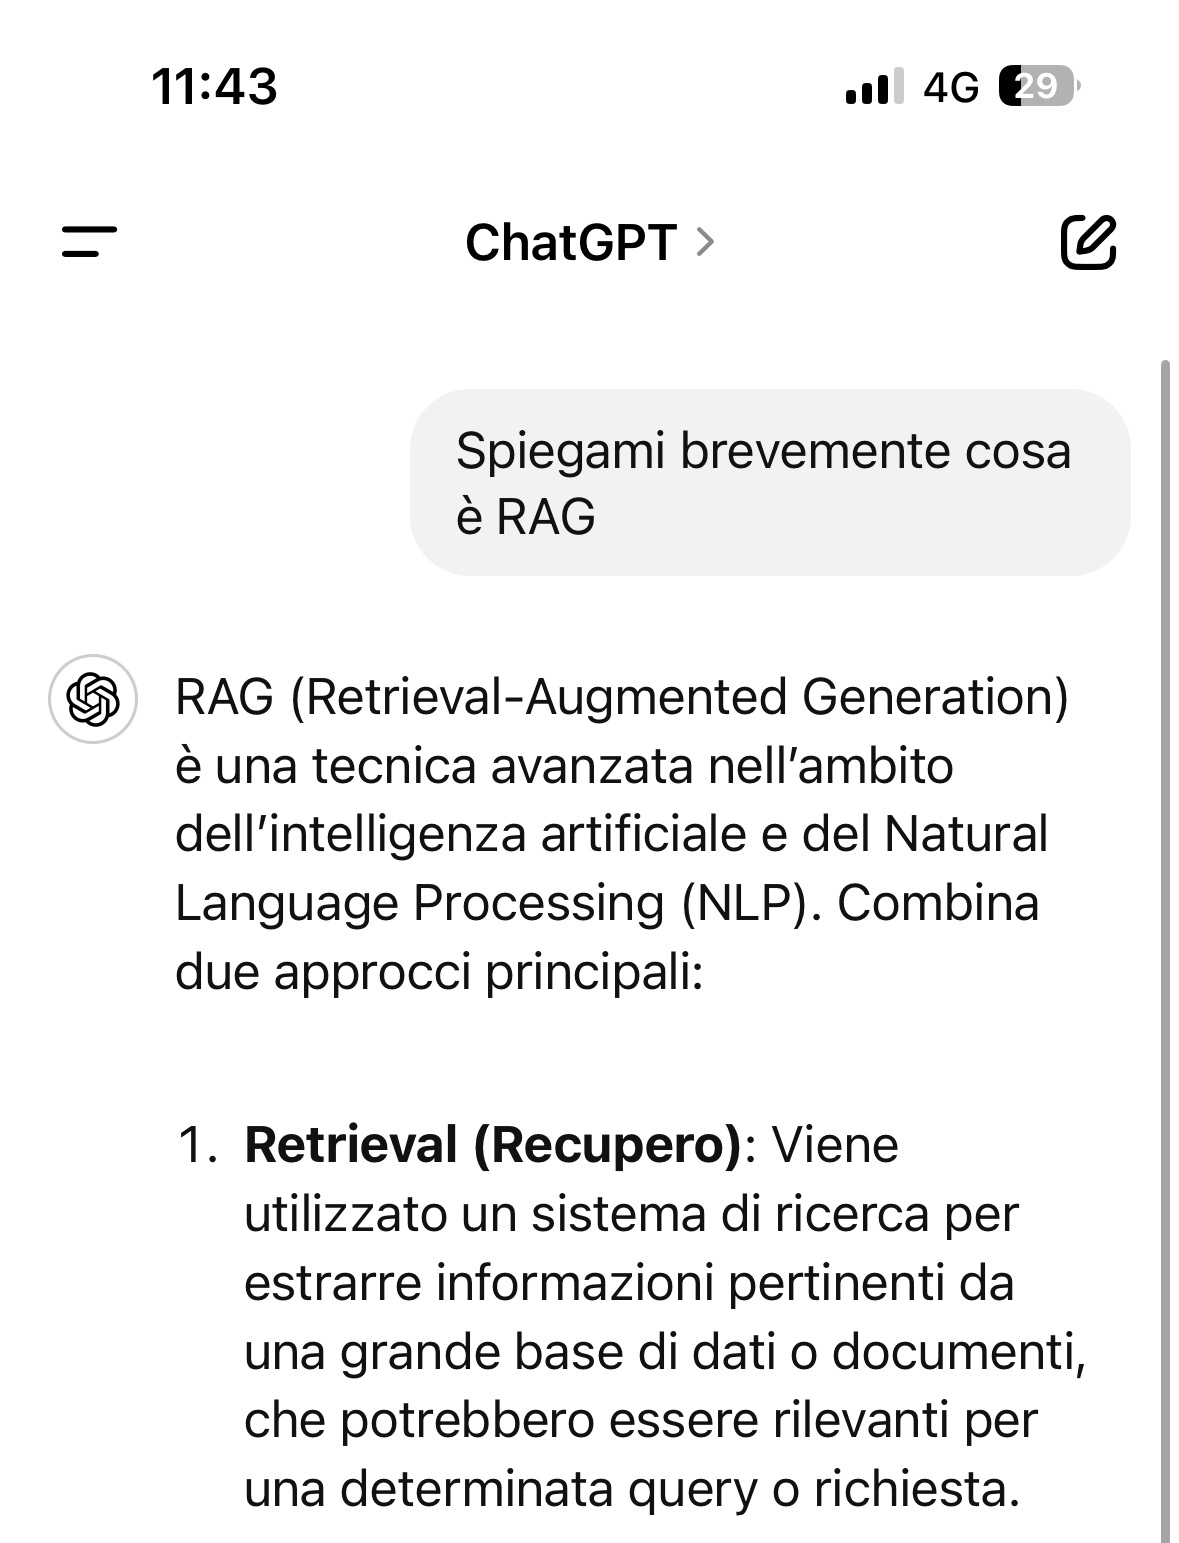
\includegraphics[width=.48\textwidth]{img/RAG_5_cut.PNG}
            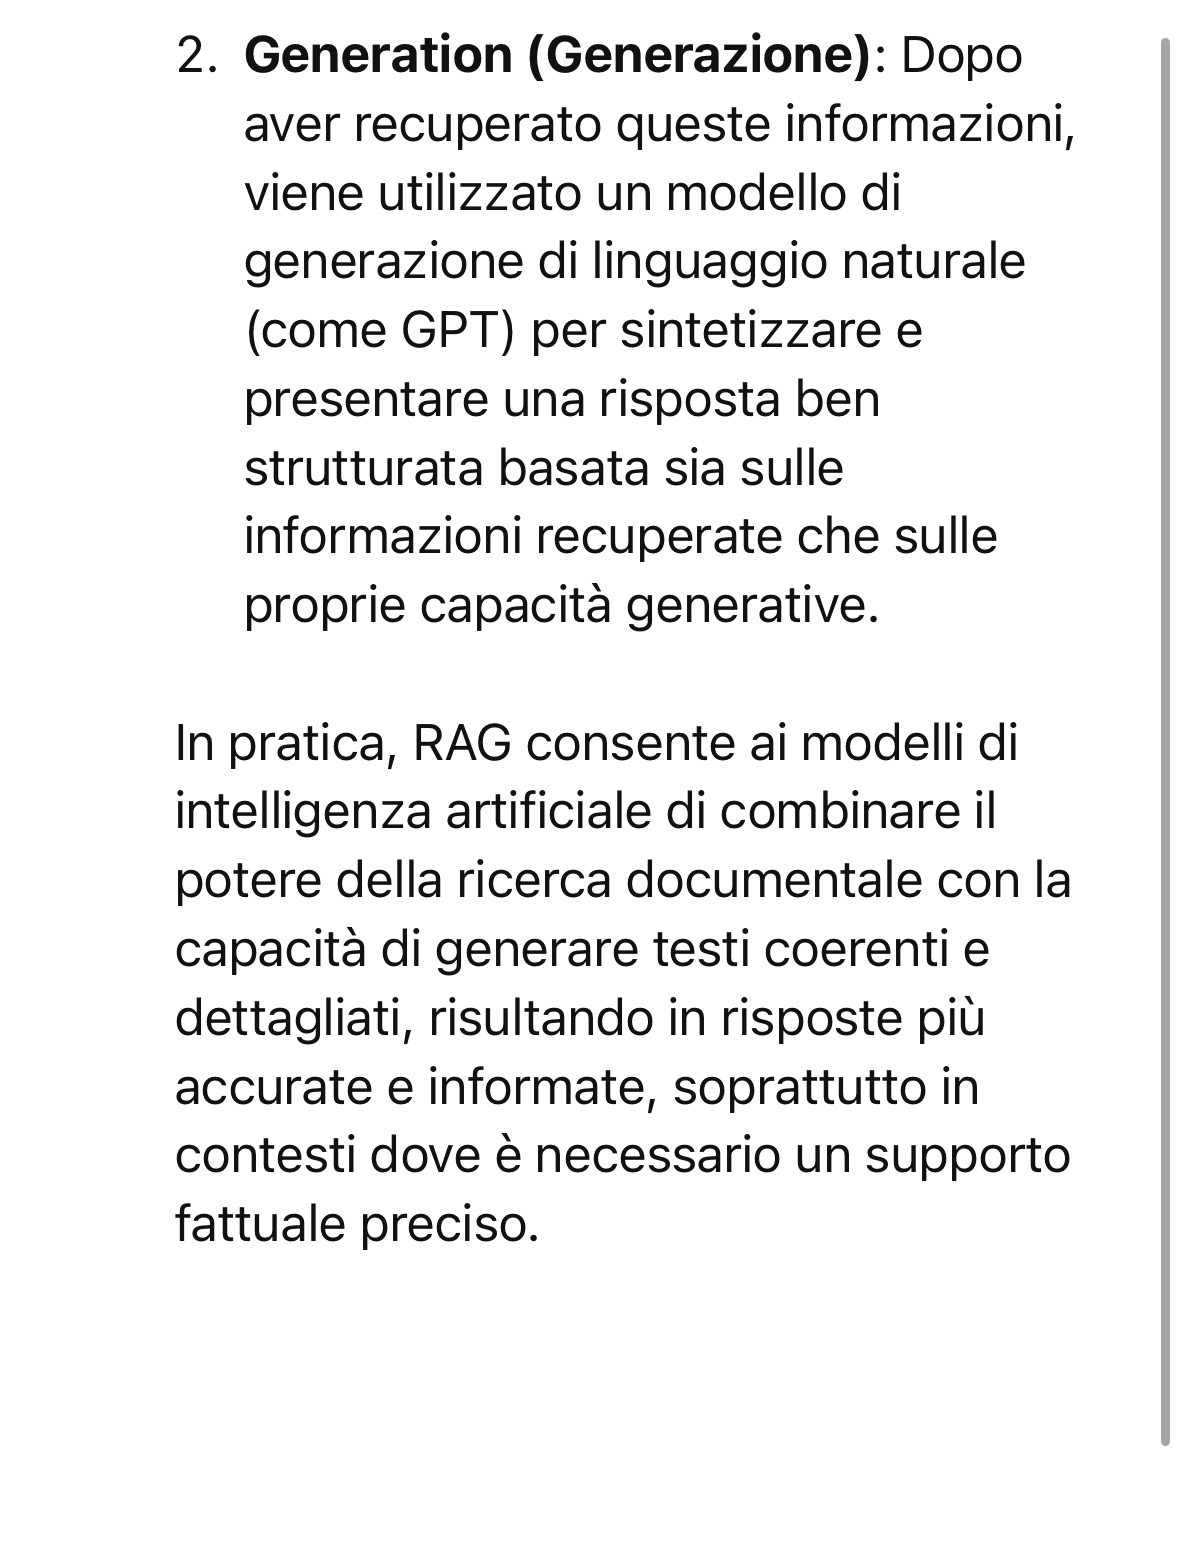
\includegraphics[width=.48\textwidth]{img/RAG_6_cut.PNG}
        \end{figure}
    \end{minipage}
    \hfill
    \begin{minipage}[t]{.35\textwidth}
        \begin{itemize}[leftmargin=10pt,align=right]
            \onslide<2->\item[\alert{\faArrowCircleRight}] Nuova frontiera del \emph{prompt engineering}
            \onslide<3->\item[\alert{\faArrowCircleRight}] Riduce i costi di addestramento LLM
            \onslide<4->\item[\alert{\faArrowCircleRight}] Mantiene costantemente aggiornati i sistemi LLM
            \onslide<5->\item[\alert{\faArrowCircleRight}] Costi di integrazione contenuti
        \end{itemize}
    \end{minipage}
}
\end{frame}
%
\begin{frame}[t] \frametitle{\emph{Retrieval Augmented Generation}}
\framesubtitle{Come funziona}
{\normalsize
    \begin{minipage}[t]{\textwidth}
        \begin{itemize}[leftmargin=10pt,align=right]
            \onslide<1->\item[\alertedcircled{1}] Utente fornisce il \textit{prompt}
            \onslide<2->\item[\alertedcircled{2}] Il sistema effettua una ricerca mirata su un \textit{data source} di informazione documentale
            \onslide<3->\item[\alertedcircled{3}] Il risultato della ricerca viene aggiunta al contesto del \textit{prompt}
        \end{itemize}
        \vspace*{.3cm}
        \begin{itemize}[leftmargin=10pt,align=right]
            \onslide<4->\item[\alert{\faExclamationTriangle}] Ricerca di tipo \alert{semantica}
            \onslide<5->\item[\alert{\faExclamationTriangle}] Solo il contesto rilevante alla richiesta aggiunto al \textit{prompt} (a differenza di \textit{chat memory}\ldots)
        \end{itemize}
    \end{minipage}
}
\end{frame}
%
\begin{frame}[t] \frametitle{\emph{Retrieval Augmented Generation}}
\framesubtitle{Vector store}
{\normalsize
    \begin{minipage}[t]{\textwidth}
        \begin{itemize}[leftmargin=10pt,align=right]
            \onslide<1->\item[\alert{\faArrowCircleRight}] Basi di dati creati per CRUD di informazione \alert{numerica multi-dimensionale}
            \onslide<2->\item[\alert{\faArrowCircleRight}] Ogni elemento nel DB è la rappresentazione numerica del suo significato (\textit{embedding})
            \begin{itemize}[leftmargin=10pt,align=right]
                \item[\alert{\faArrowCircleRight}] Testi
                \item[\alert{\faArrowCircleRight}] Immagini
                \item[\alert{\faArrowCircleRight}] Video
                \item[\alert{\faArrowCircleRight}] Audio
                \item[\alert{\faArrowCircleRight}] \ldots
            \end{itemize}
            \onslide<3->\item[\alert{\faArrowCircleRight}] Evoluzioni dei DB ottimizzati per ricerca su \textit{keyword} (es. ElasticSearch)
            \begin{itemize}[leftmargin=10pt,align=right]
                \item[\alert{\faExclamationTriangle}] Non più limitati alla ricerca per parola esatta/simile!
            \end{itemize}
        \end{itemize}
    \end{minipage}
}
\end{frame}
%
\begin{frame}[t] \frametitle{\emph{Retrieval Augmented Generation}}
\framesubtitle{Famiglie di vector store}
{\normalsize
    \begin{minipage}[t]{\textwidth}
        \begin{itemize}[leftmargin=10pt,align=right]
            \onslide<1->\item[\alert{\faArrowCircleRight}] \textit{Data source} nativi
            \begin{itemize}[leftmargin=10pt,align=right]
                \item[\alert{\faArrowCircleRight}] Qdrant
                \item[\alert{\faArrowCircleRight}] ChromaDB
                \item[\alert{\faArrowCircleRight}] Neo4j
                \item[\alert{\faArrowCircleRight}] \ldots
            \end{itemize}
            \onslide<2-> \textit{Data source} SQL/noSQL con interazione \textit{vector data storage}
            \begin{itemize}[leftmargin=10pt,align=right]
                \item[\alert{\faArrowCircleRight}] MongoDB
                \item[\alert{\faArrowCircleRight}] PostgreSQL + pgvector
                \item[\alert{\faArrowCircleRight}] Redis + RediSearch
                \item[\alert{\faArrowCircleRight}] ElasticSearch
                \item[\alert{\faArrowCircleRight}] \ldots
            \end{itemize}
        \end{itemize}
    \end{minipage}
}
\end{frame}
%
\begin{frame}[t] \frametitle{\emph{Workflow} del processo RAG}
{\scriptsize
\only<1>{
    \framesubtitle{Approccio non generativo}
    \begin{center}
        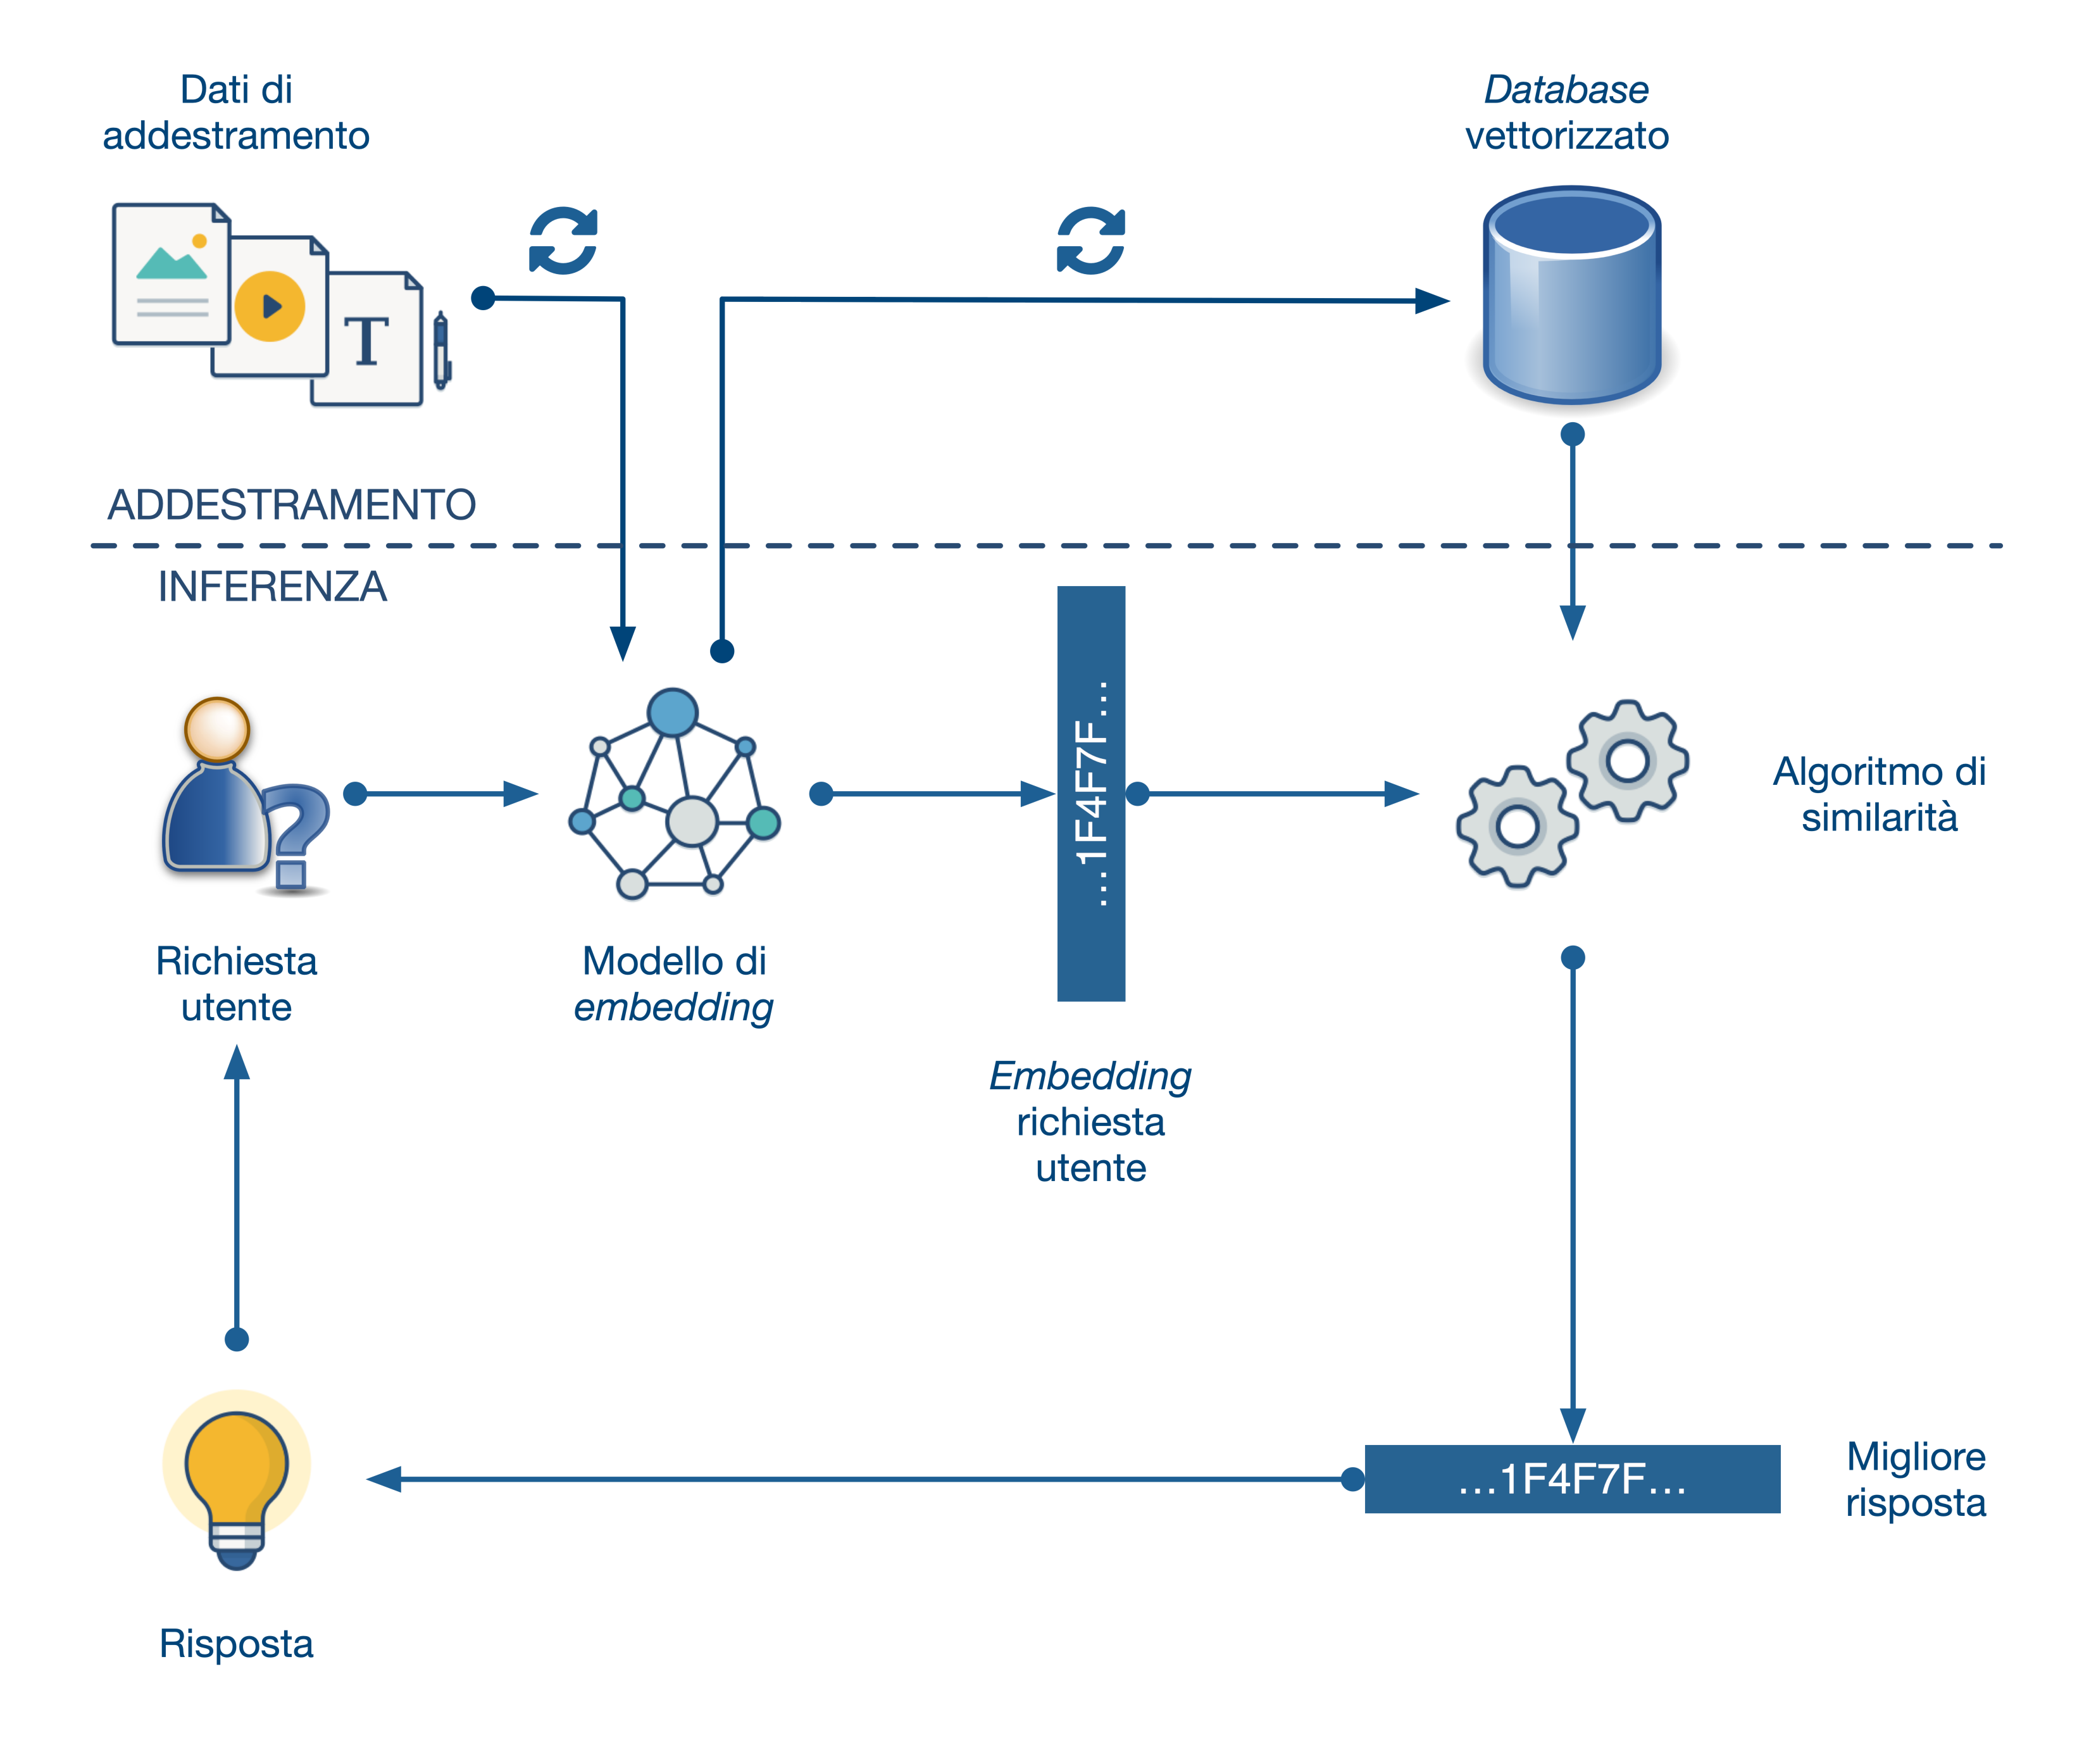
\includegraphics[width=.75\textwidth]{img/RAG-no-LLM-scaled.png}
    \end{center}
}
\only<2->{
    \framesubtitle{Approccio generativo}
    \begin{center}
        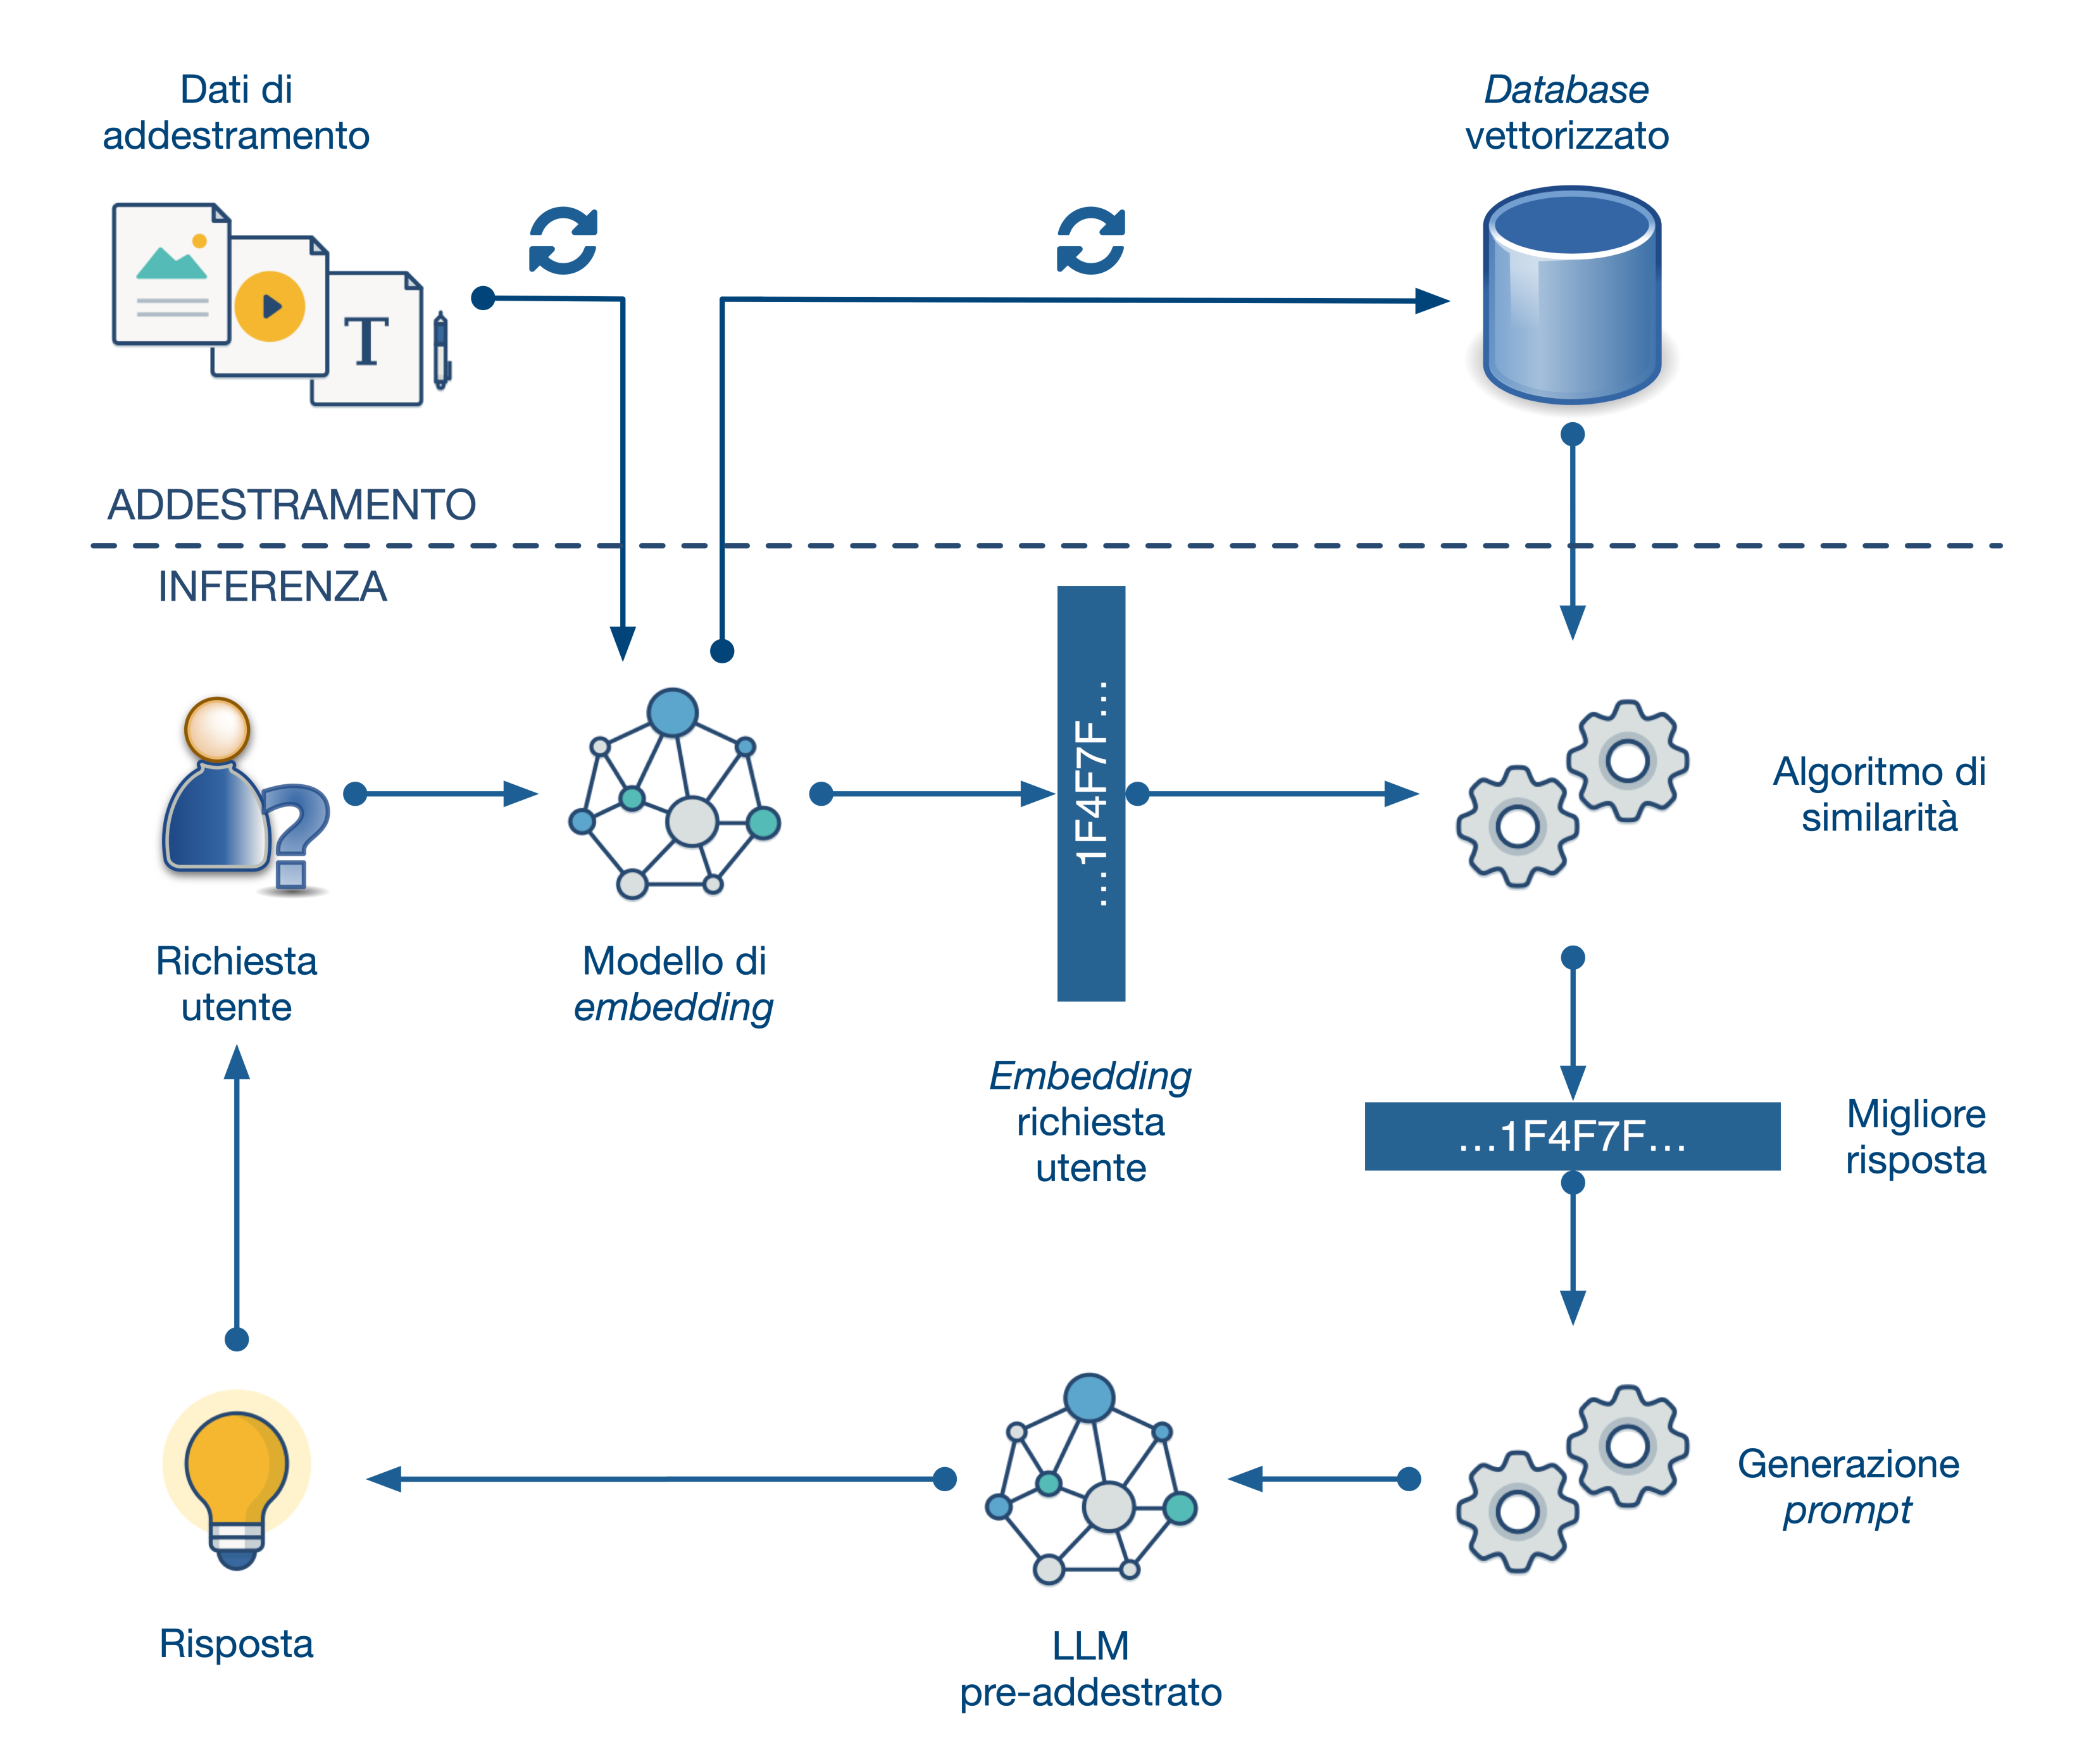
\includegraphics[width=.75\textwidth]{img/RAG-LLM-scaled.png}
    \end{center}
}
}
\end{frame}
%
\begin{frame}[t] \frametitle{RAG non generativo: esempio}
{\scriptsize
\framesubtitle{Ricerca semantica di film e serie}
\only<1>{
    \begin{center}
        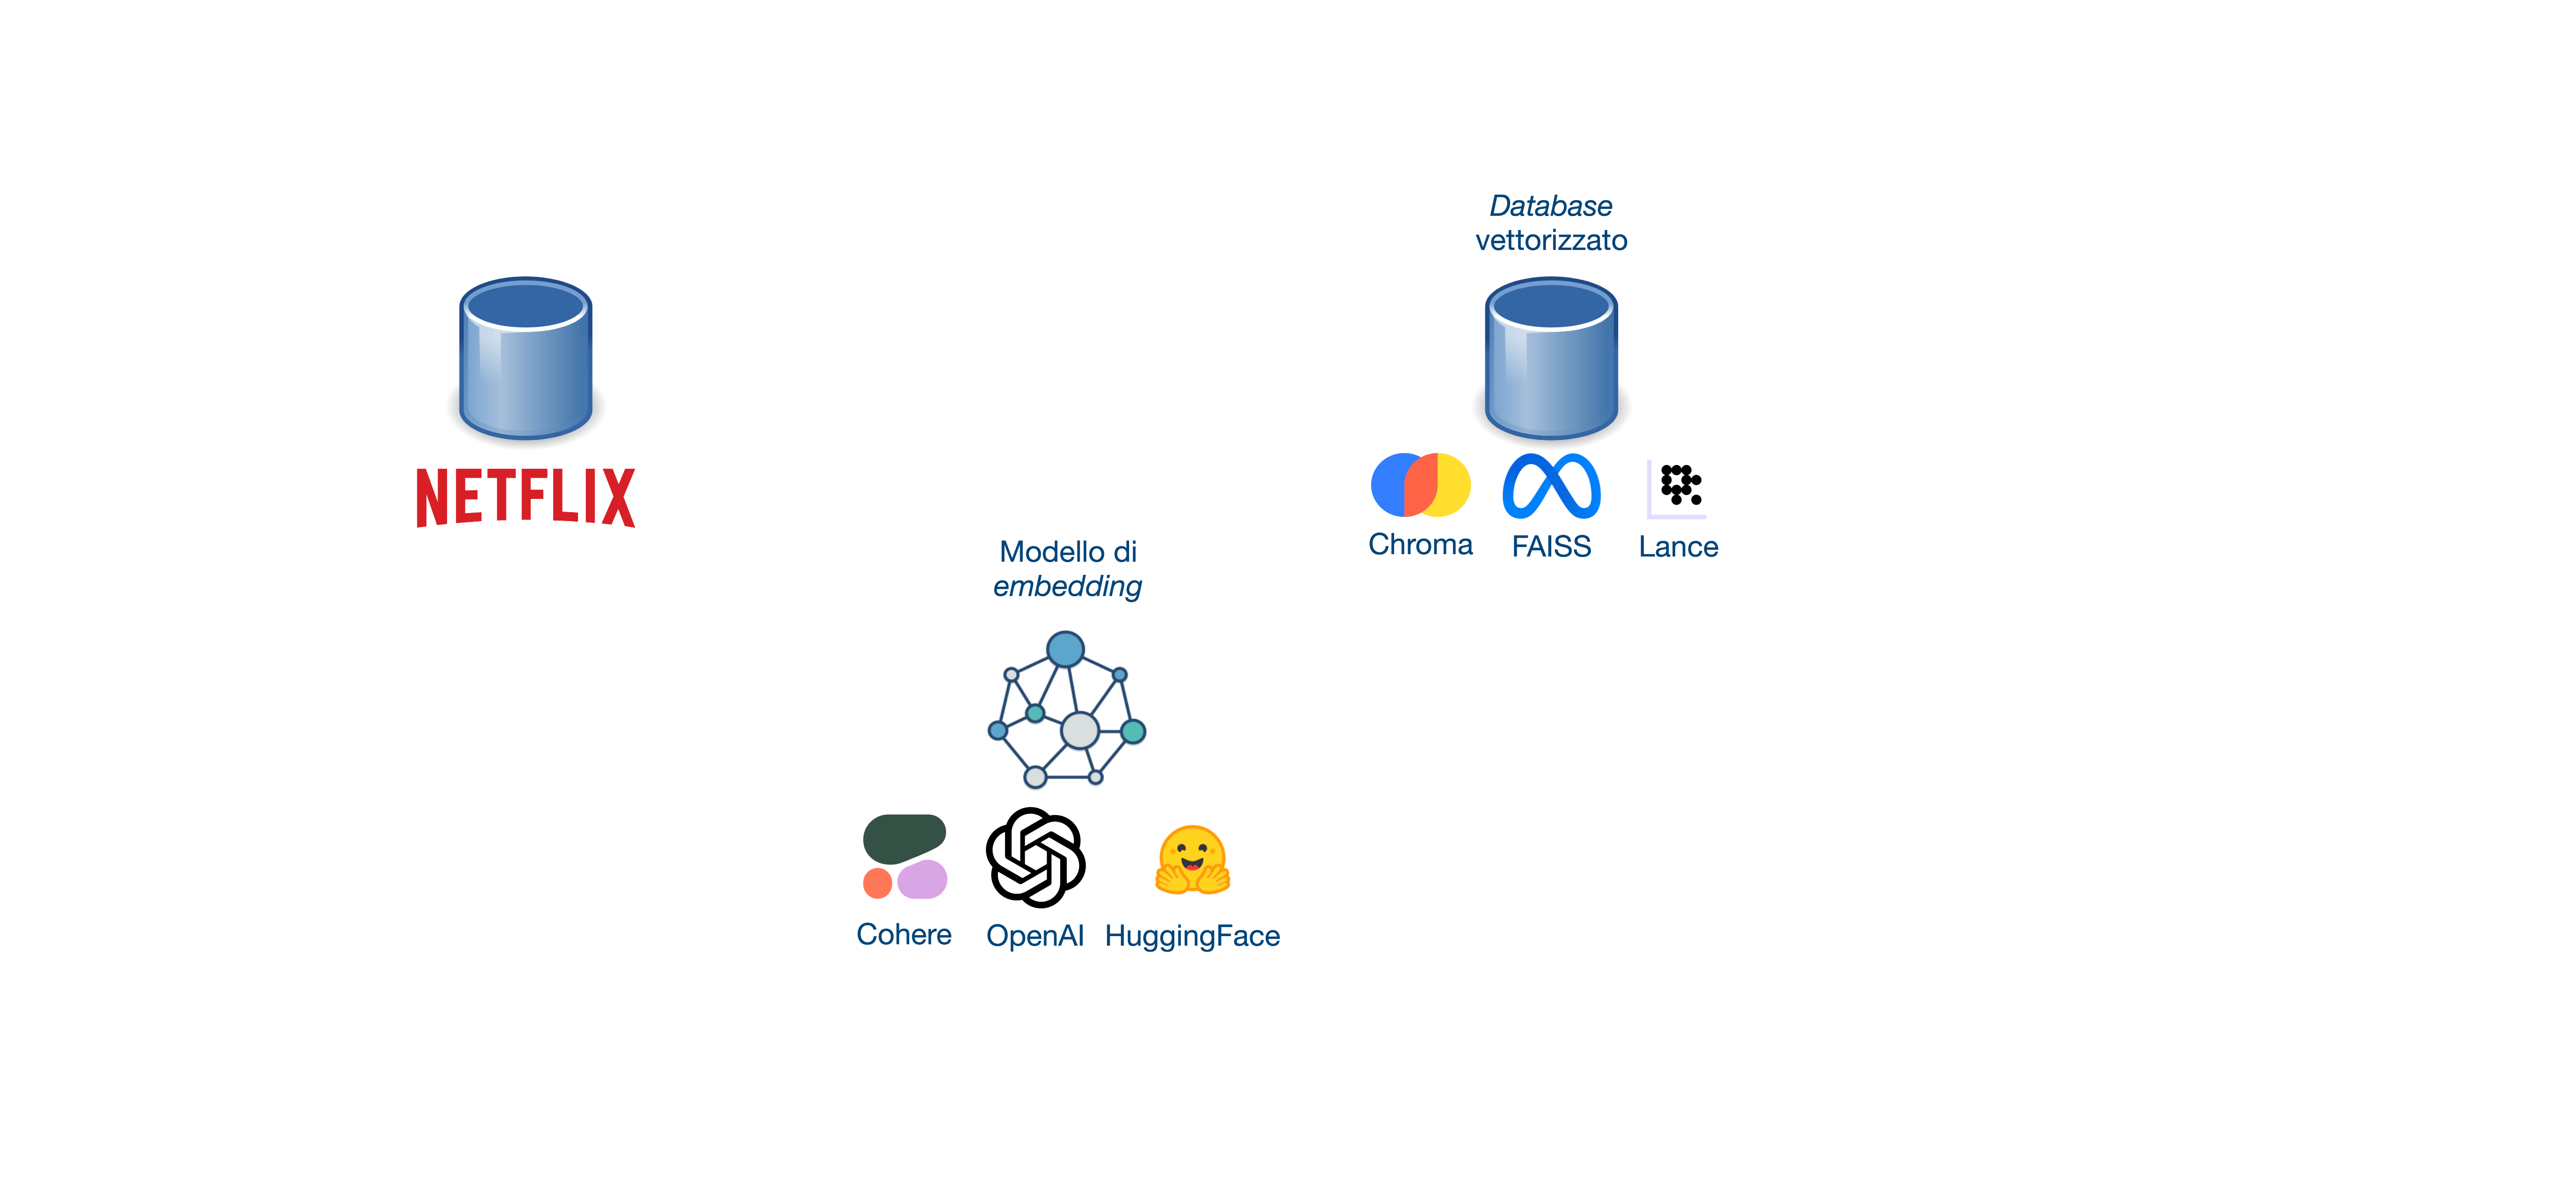
\includegraphics[width=\textwidth]{img/RAG-NO-LLM-NETFLIX-0-scaled.png}
    \end{center}
}
    \only<2>{
    \begin{center}
        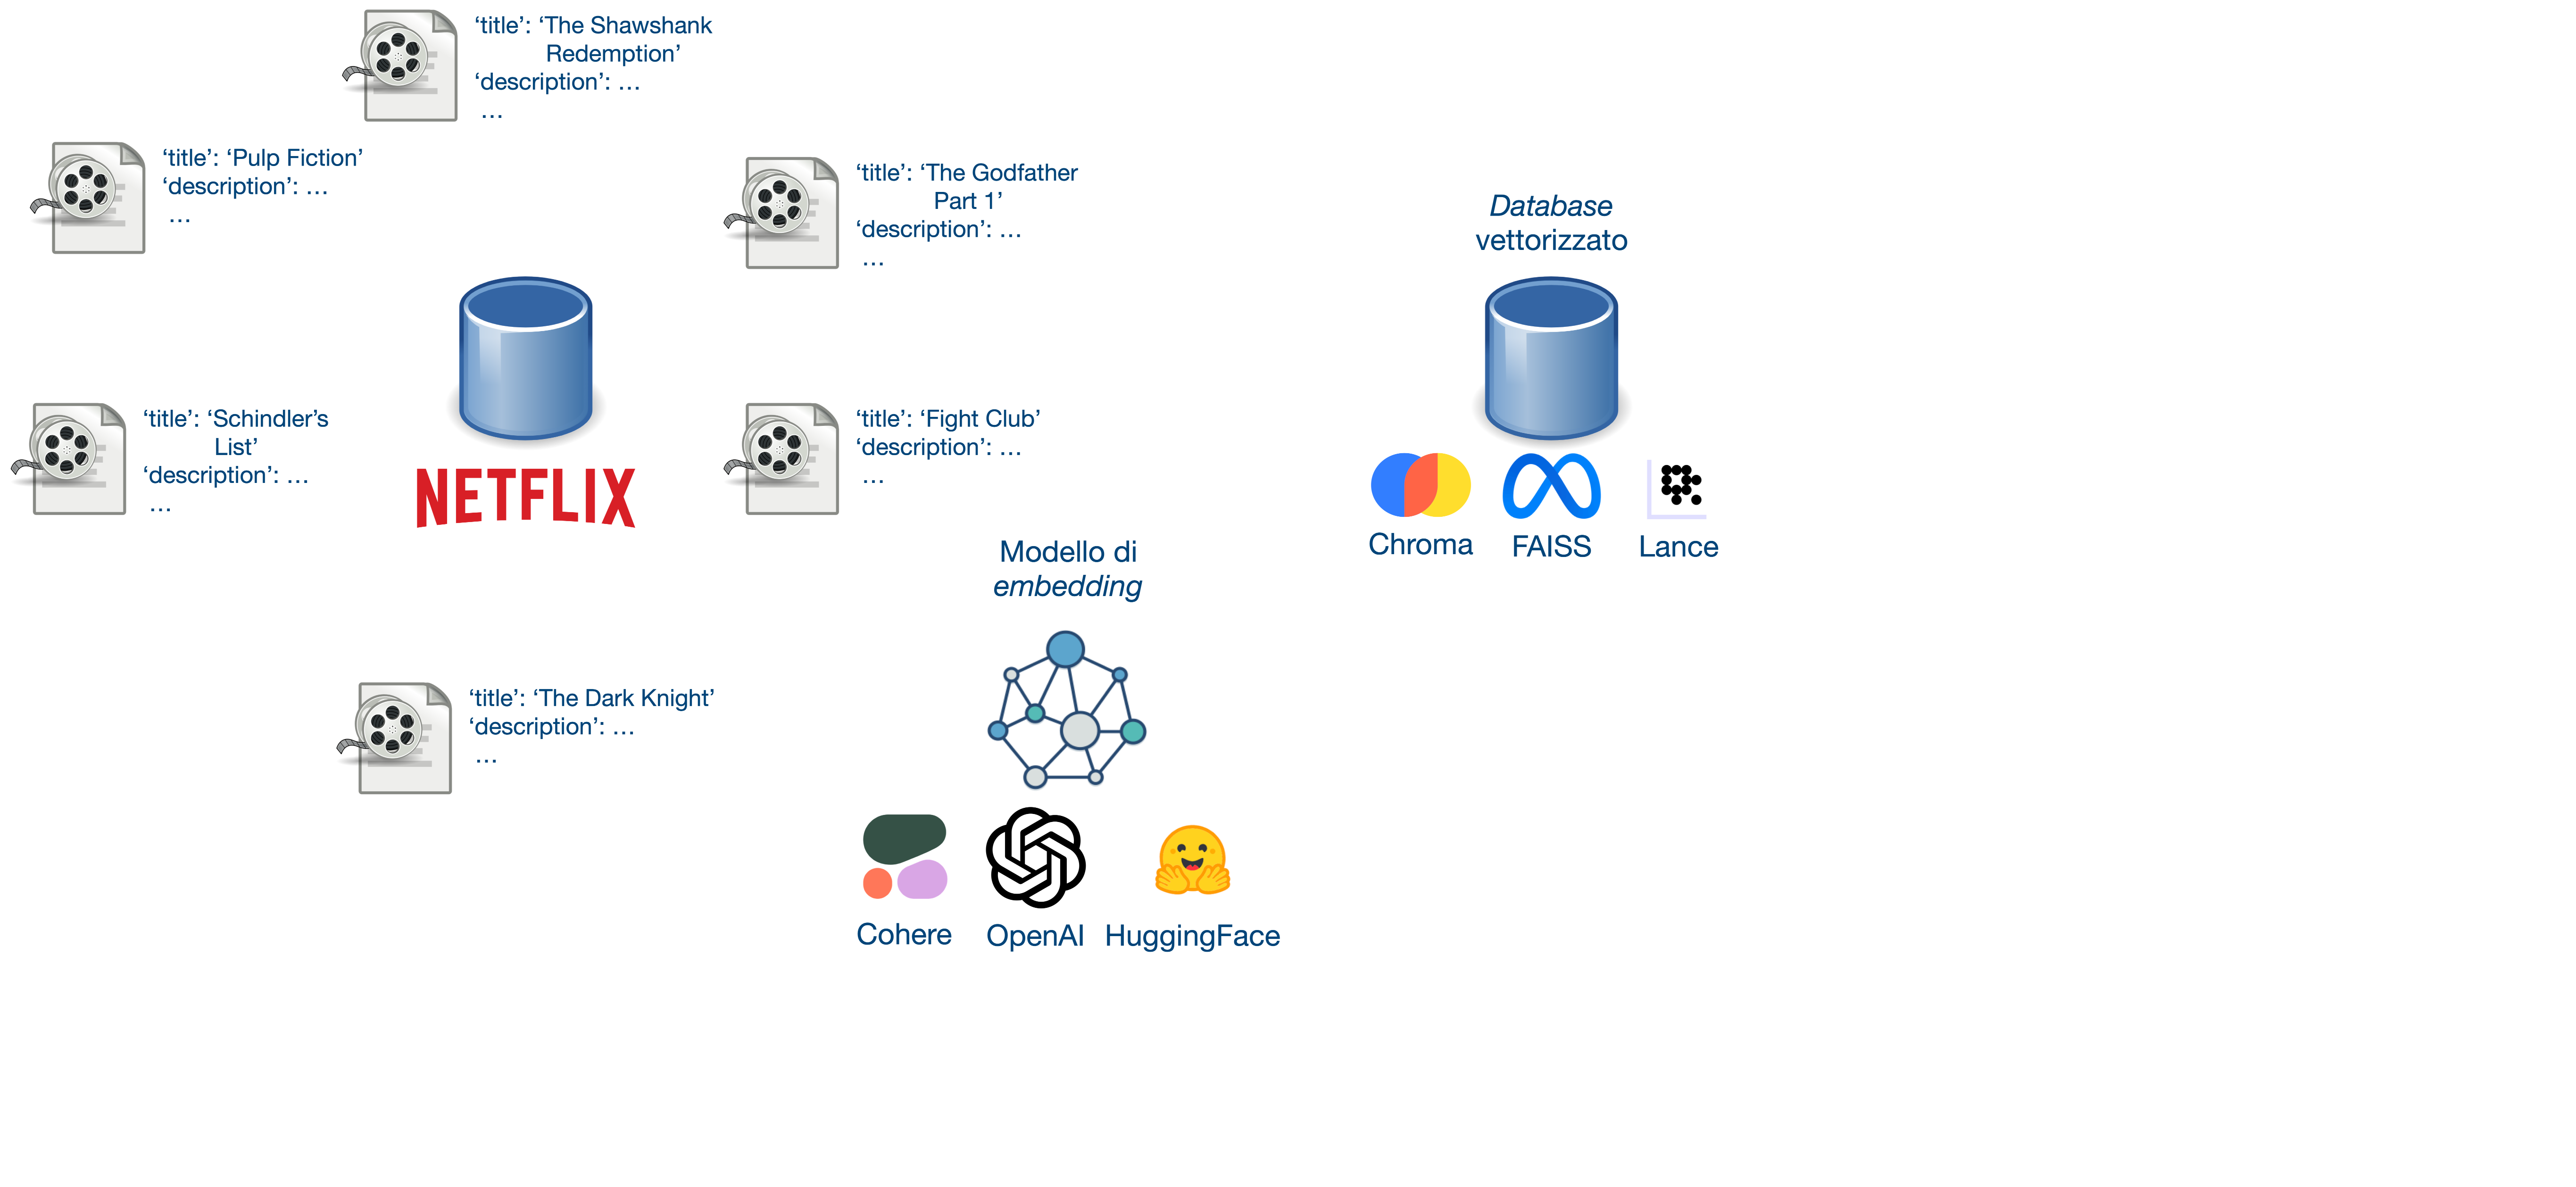
\includegraphics[width=\textwidth]{img/RAG-NO-LLM-NETFLIX-1-scaled.png}
    \end{center}
}
    \only<3>{
    \begin{center}
        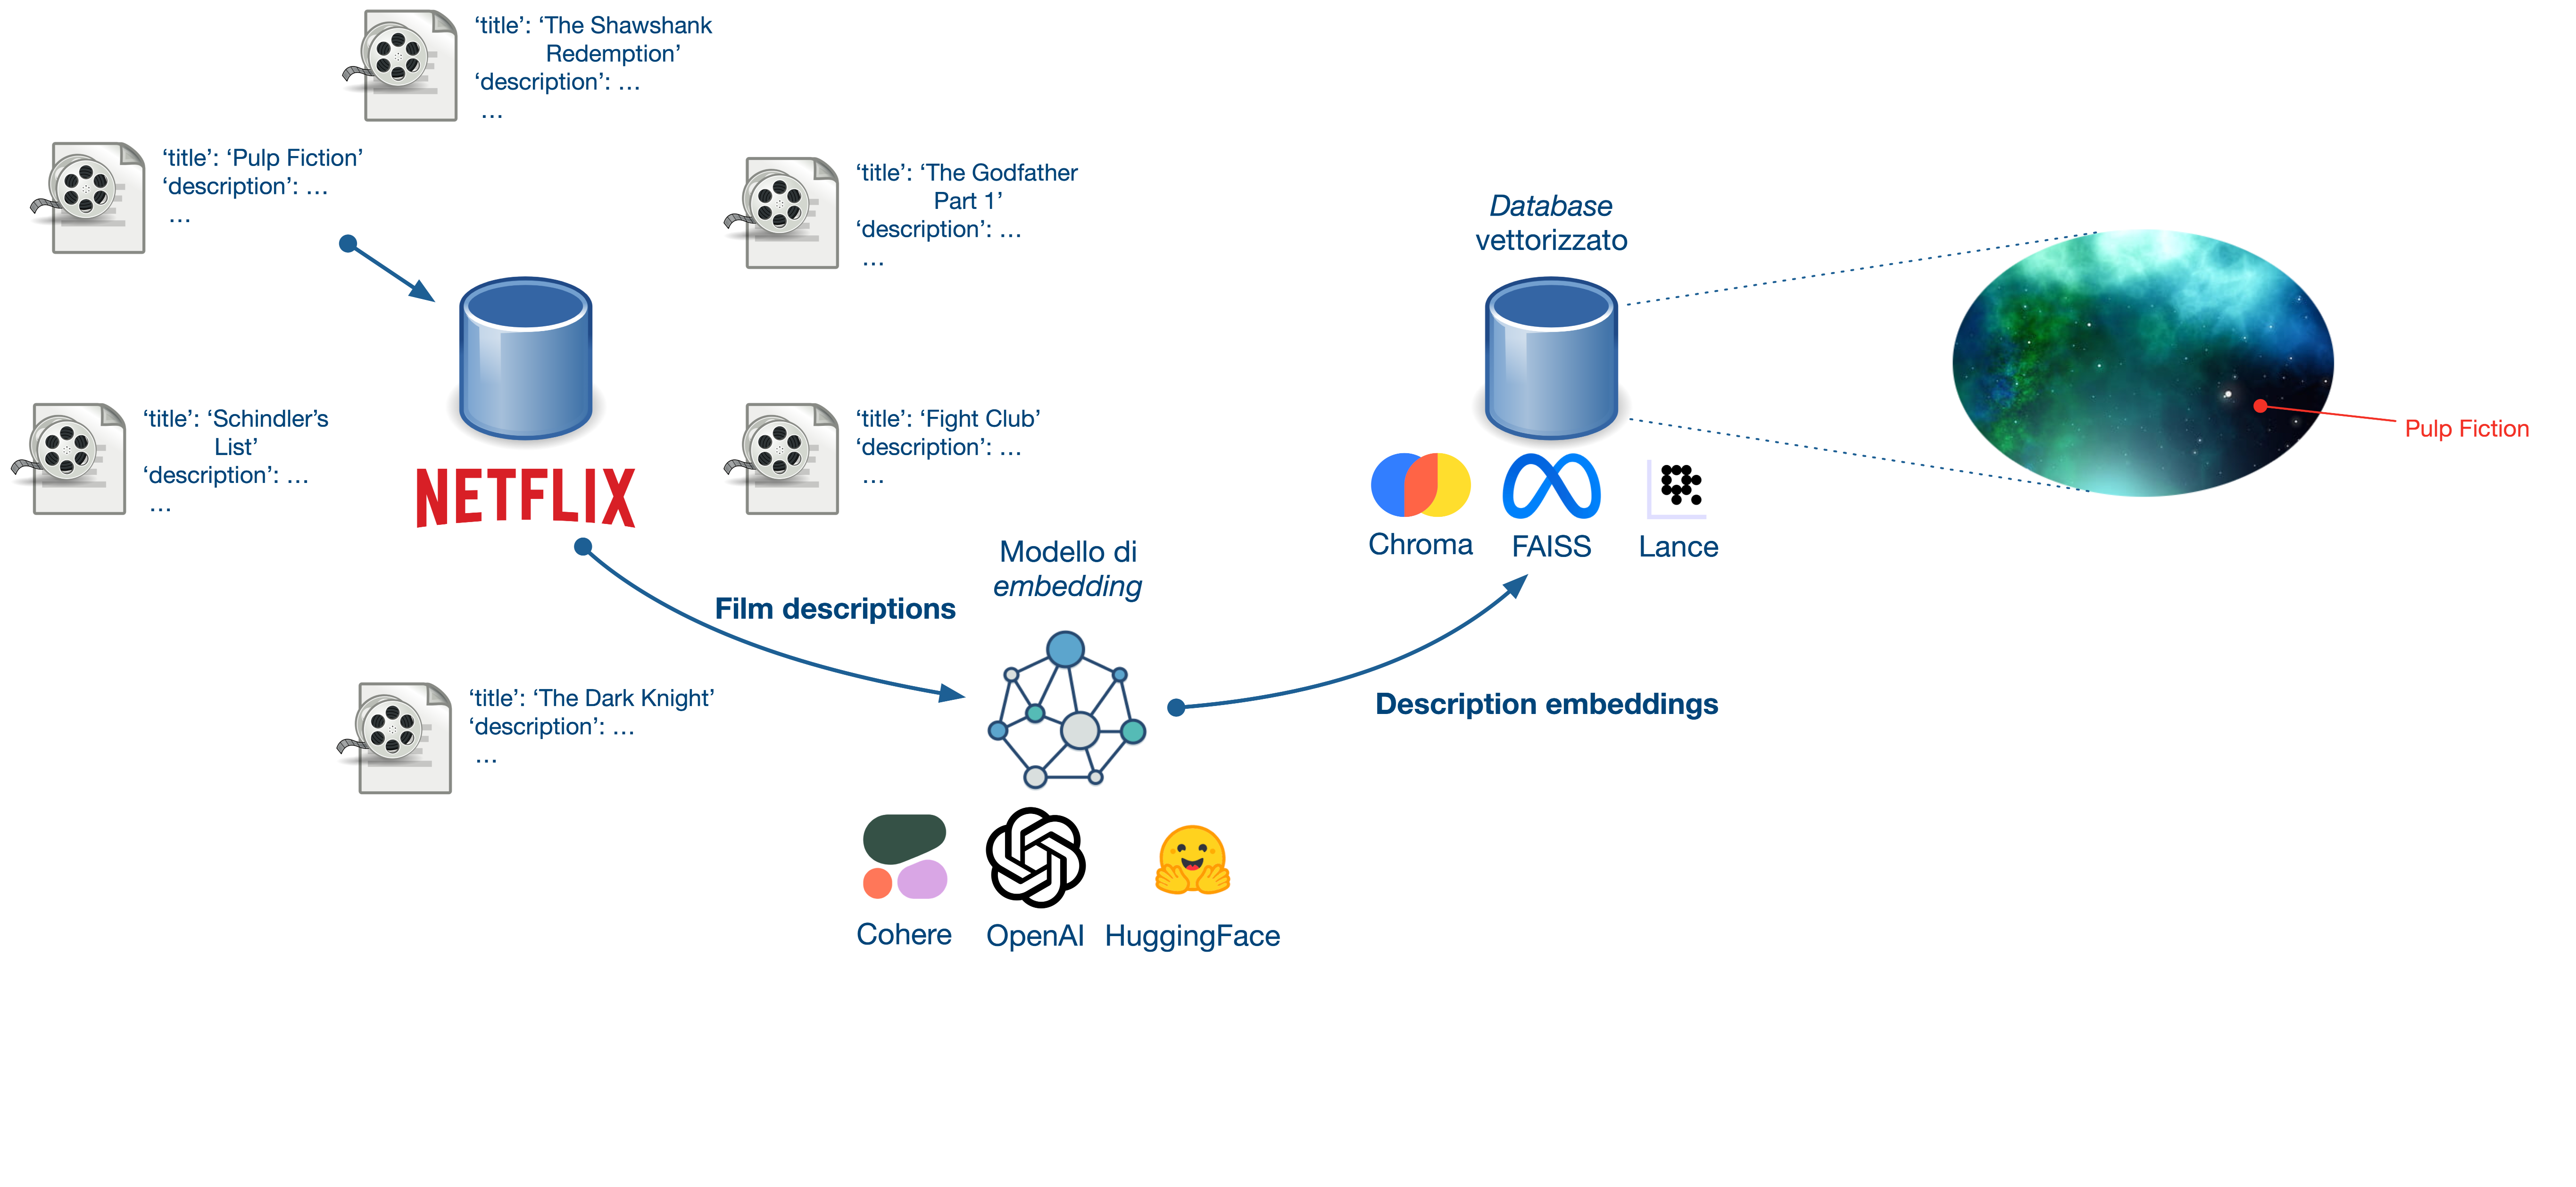
\includegraphics[width=\textwidth]{img/RAG-NO-LLM-NETFLIX-2-scaled.png}
    \end{center}
}
    \only<4>{
    \begin{center}
        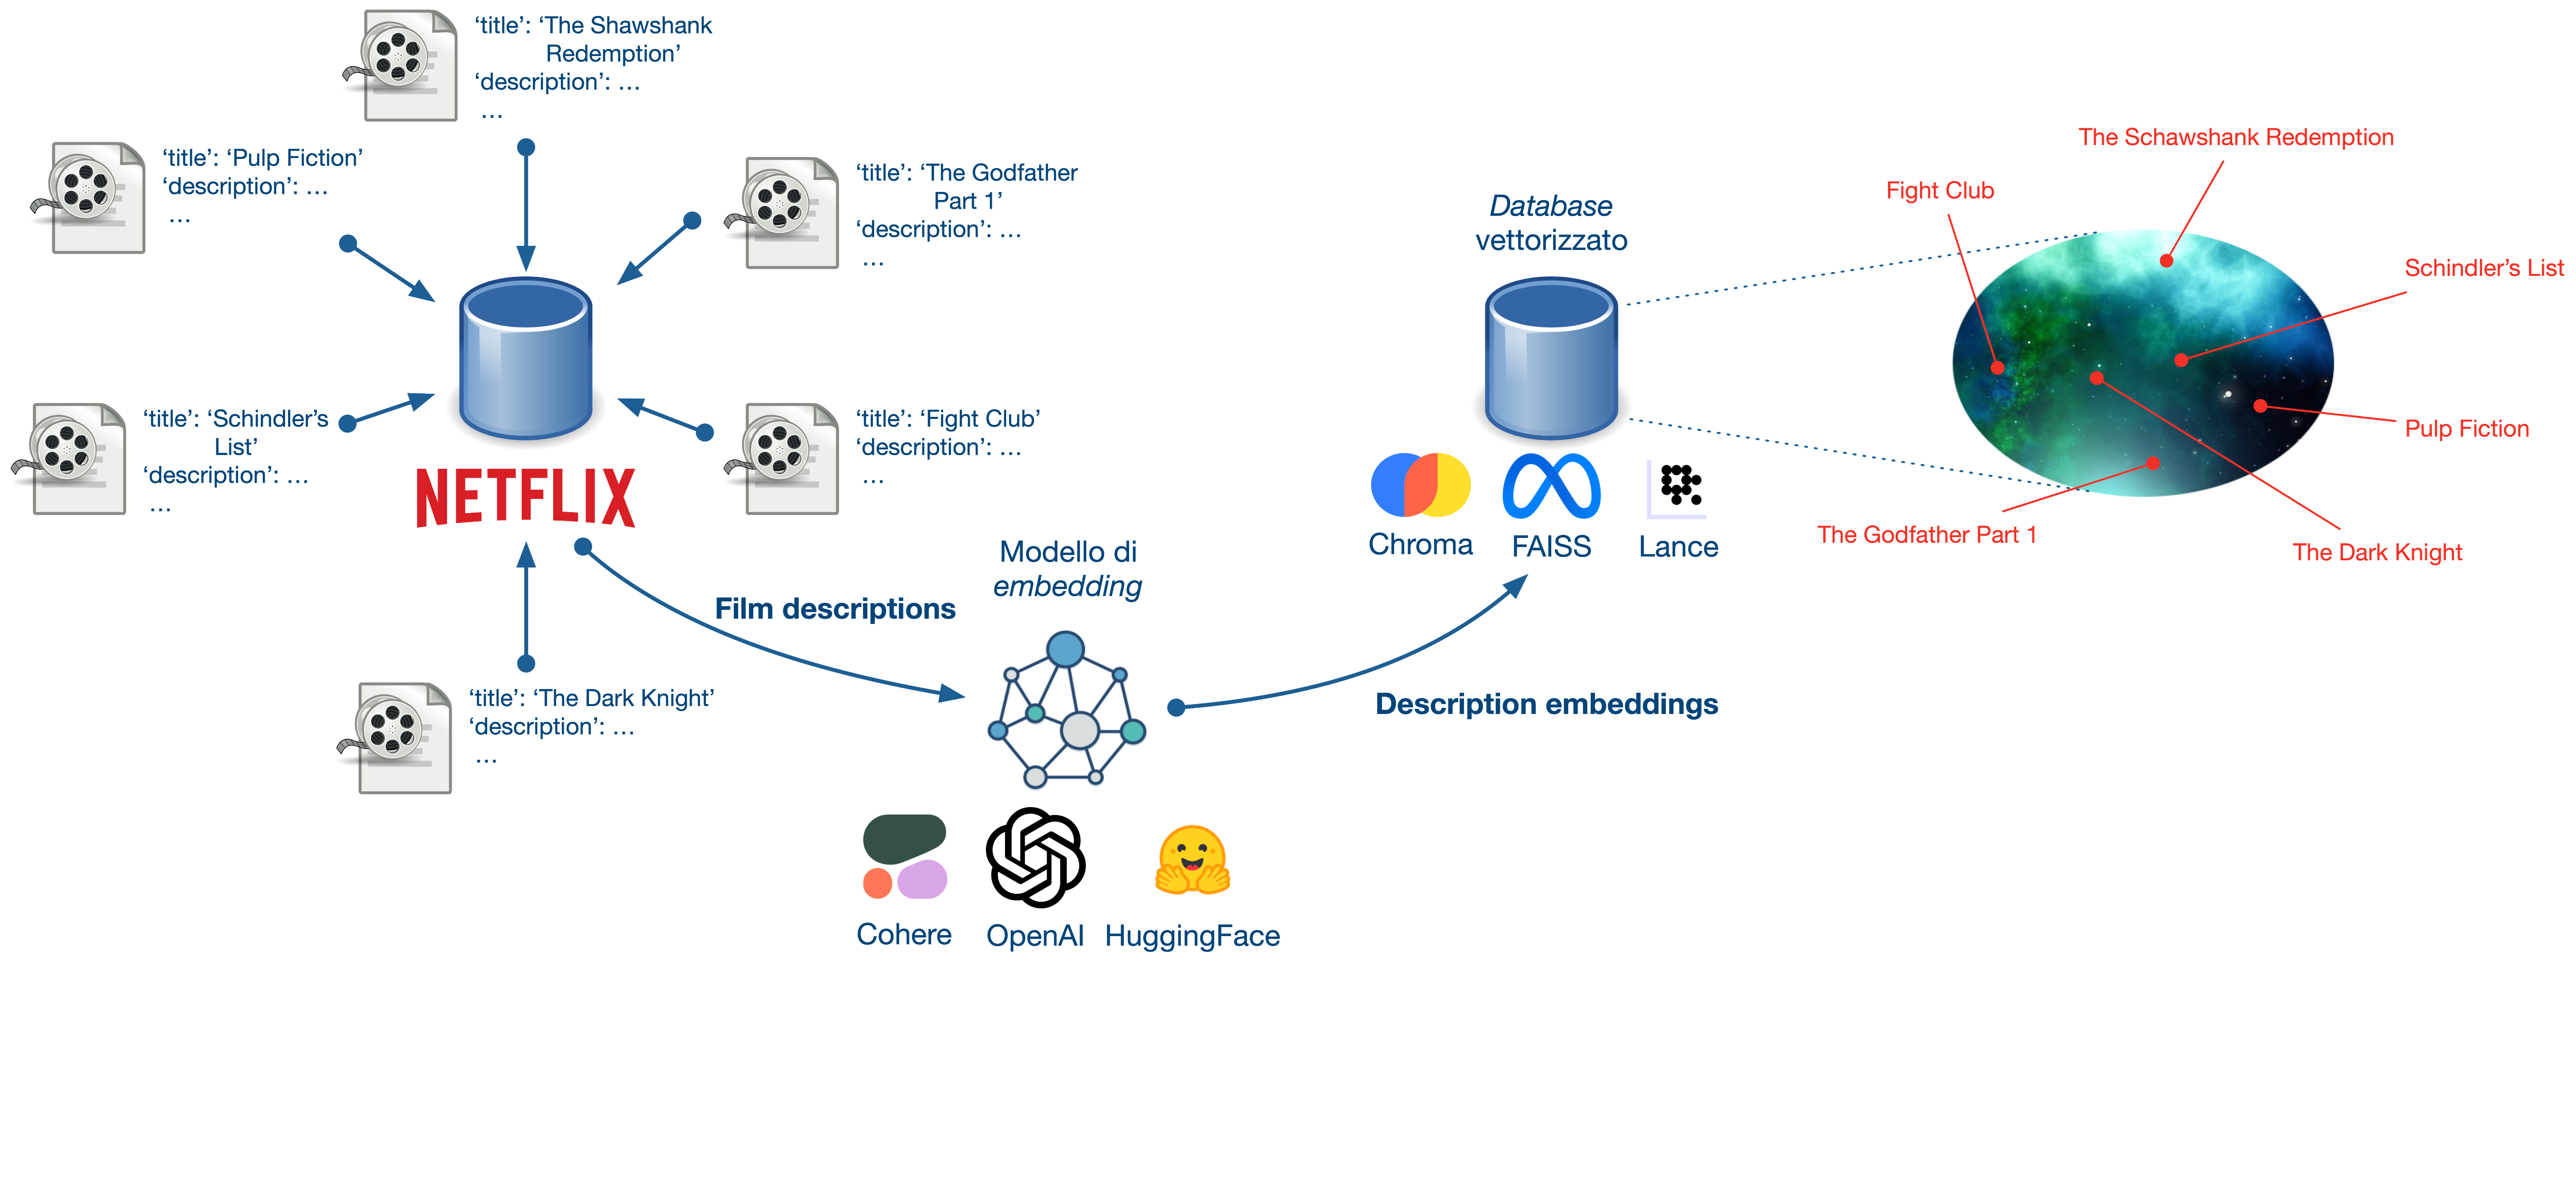
\includegraphics[width=\textwidth]{img/RAG-NO-LLM-NETFLIX-3-scaled.png}
    \end{center}
}
    \only<5>{
    \begin{center}
        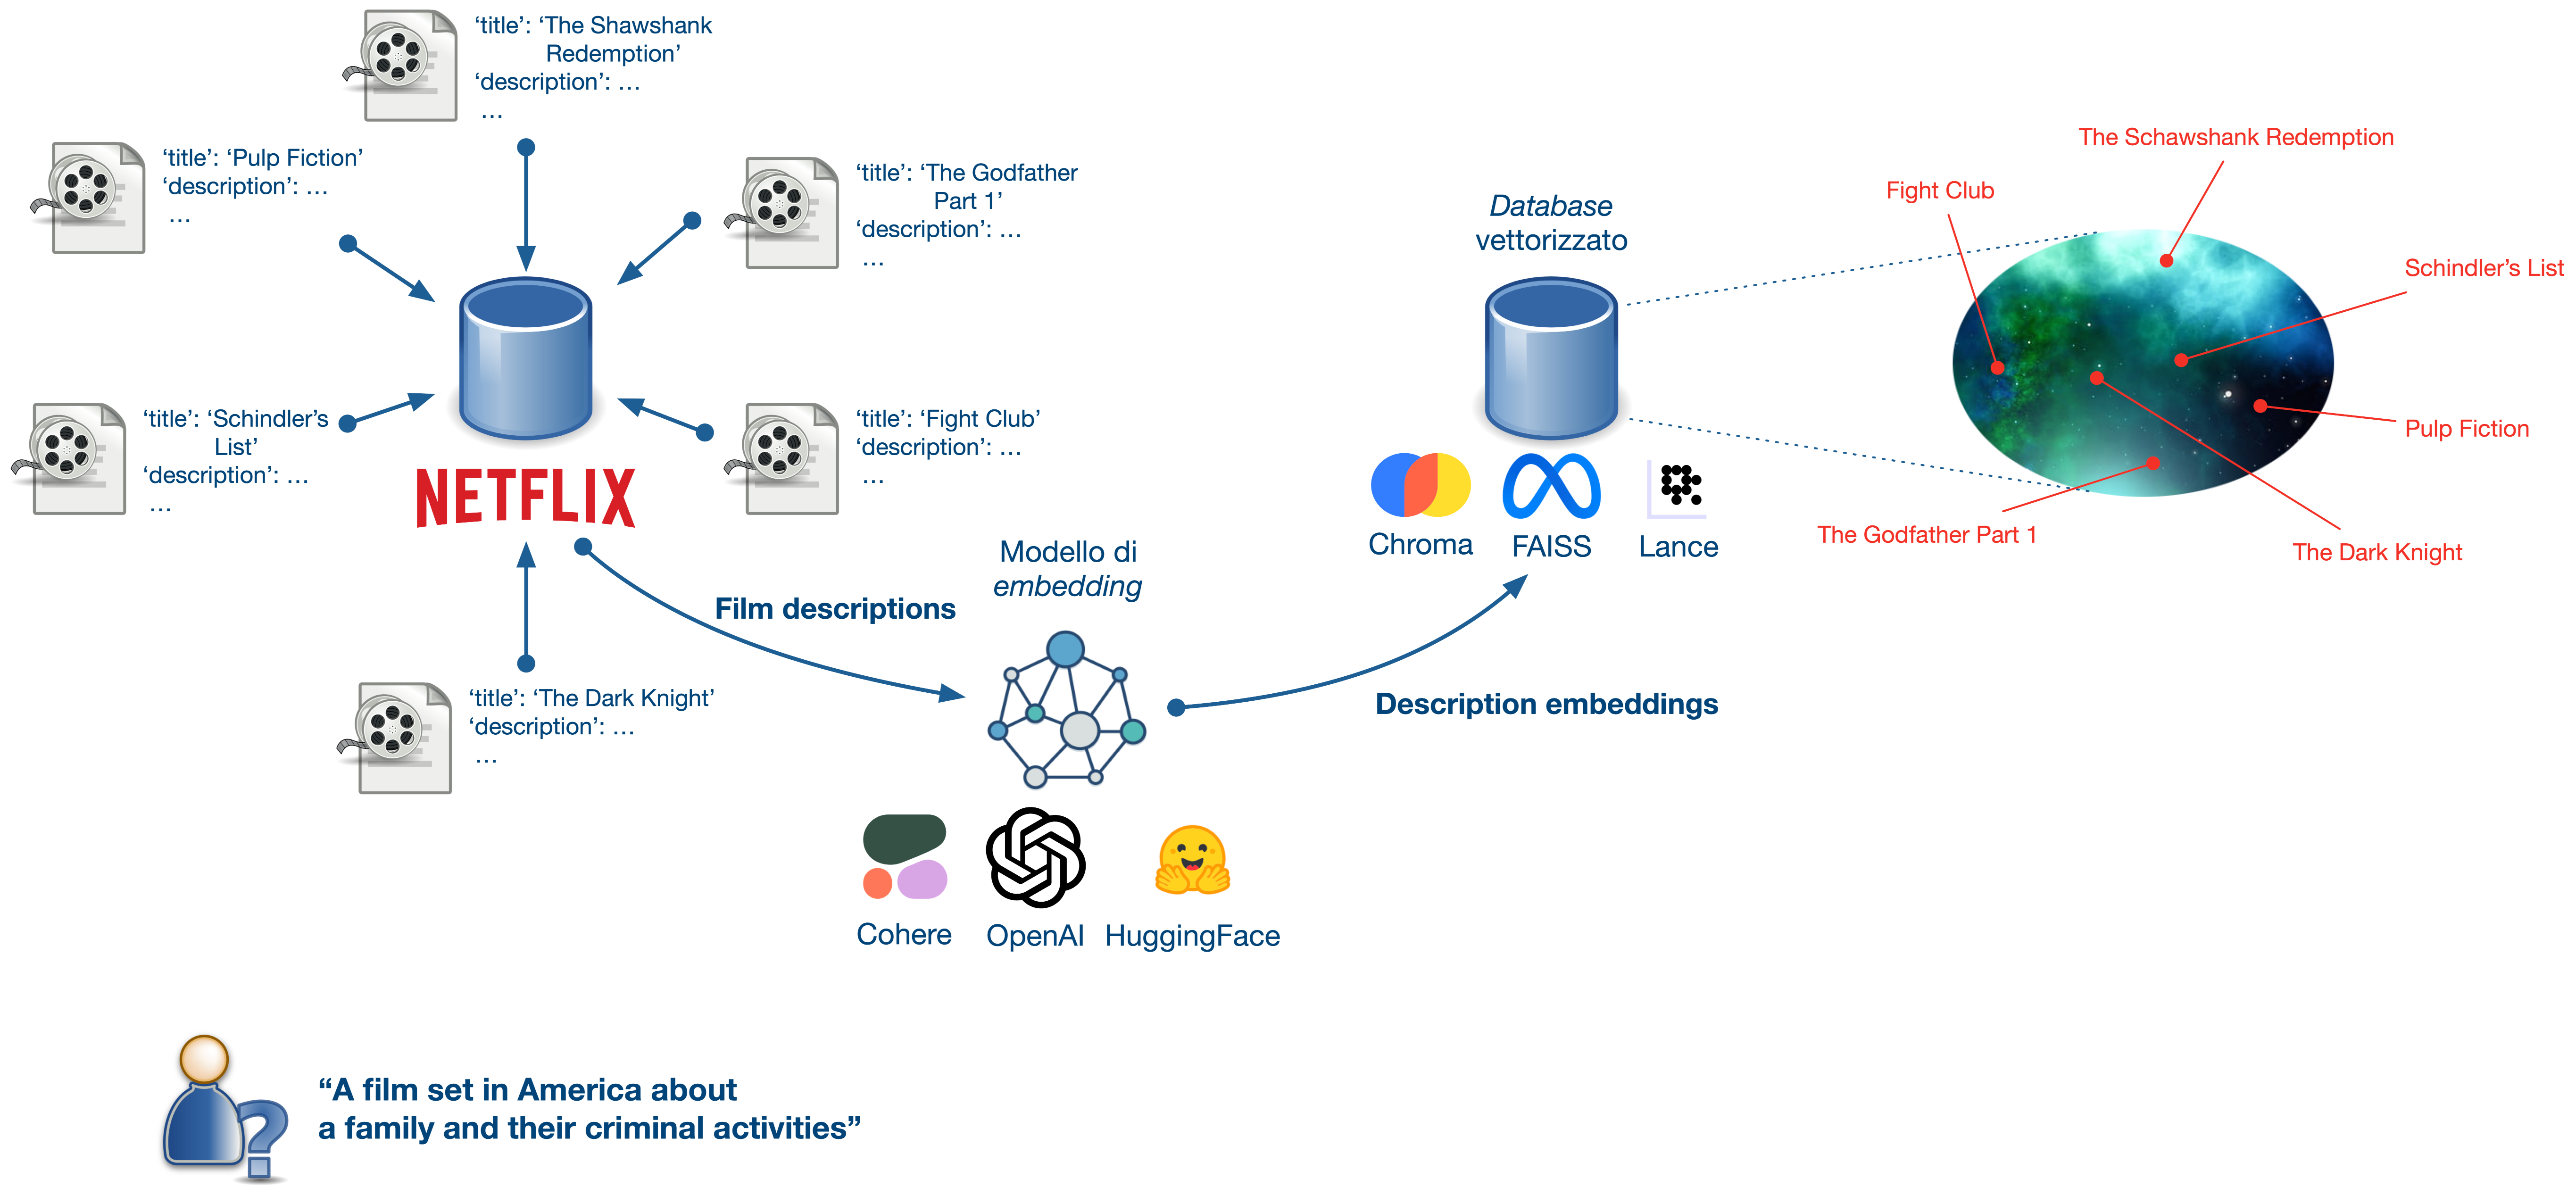
\includegraphics[width=\textwidth]{img/RAG-NO-LLM-NETFLIX-4-scaled.png}
    \end{center}
}
    \only<6>{
    \begin{center}
        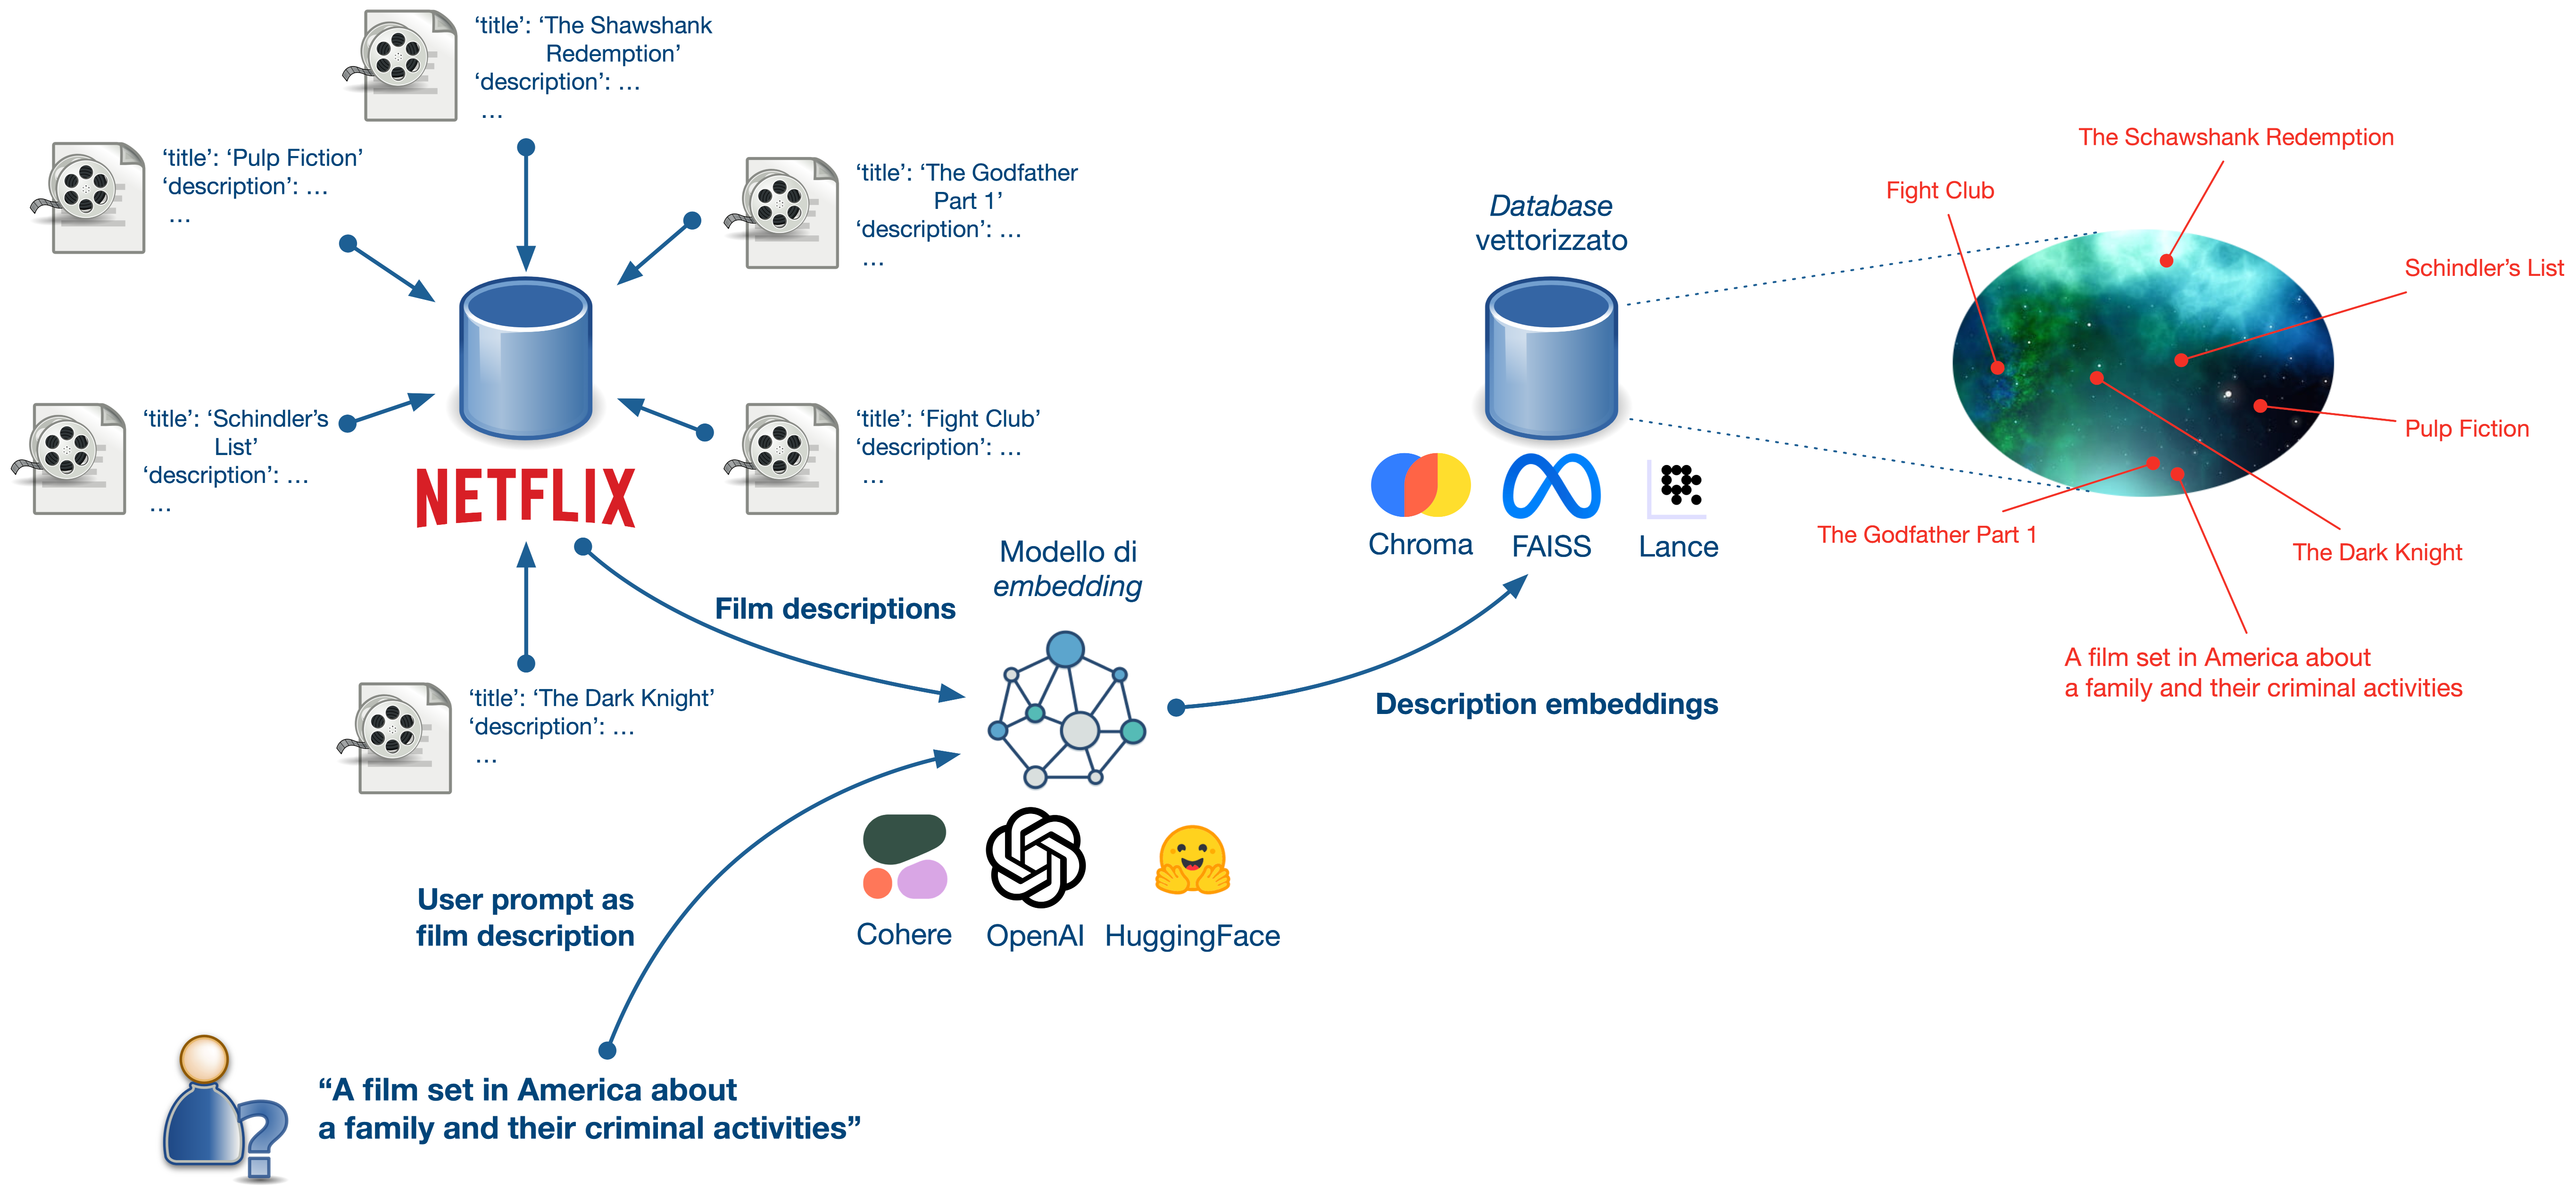
\includegraphics[width=\textwidth]{img/RAG-NO-LLM-NETFLIX-5-scaled.png}
    \end{center}
}
    \only<7>{
    \begin{center}
        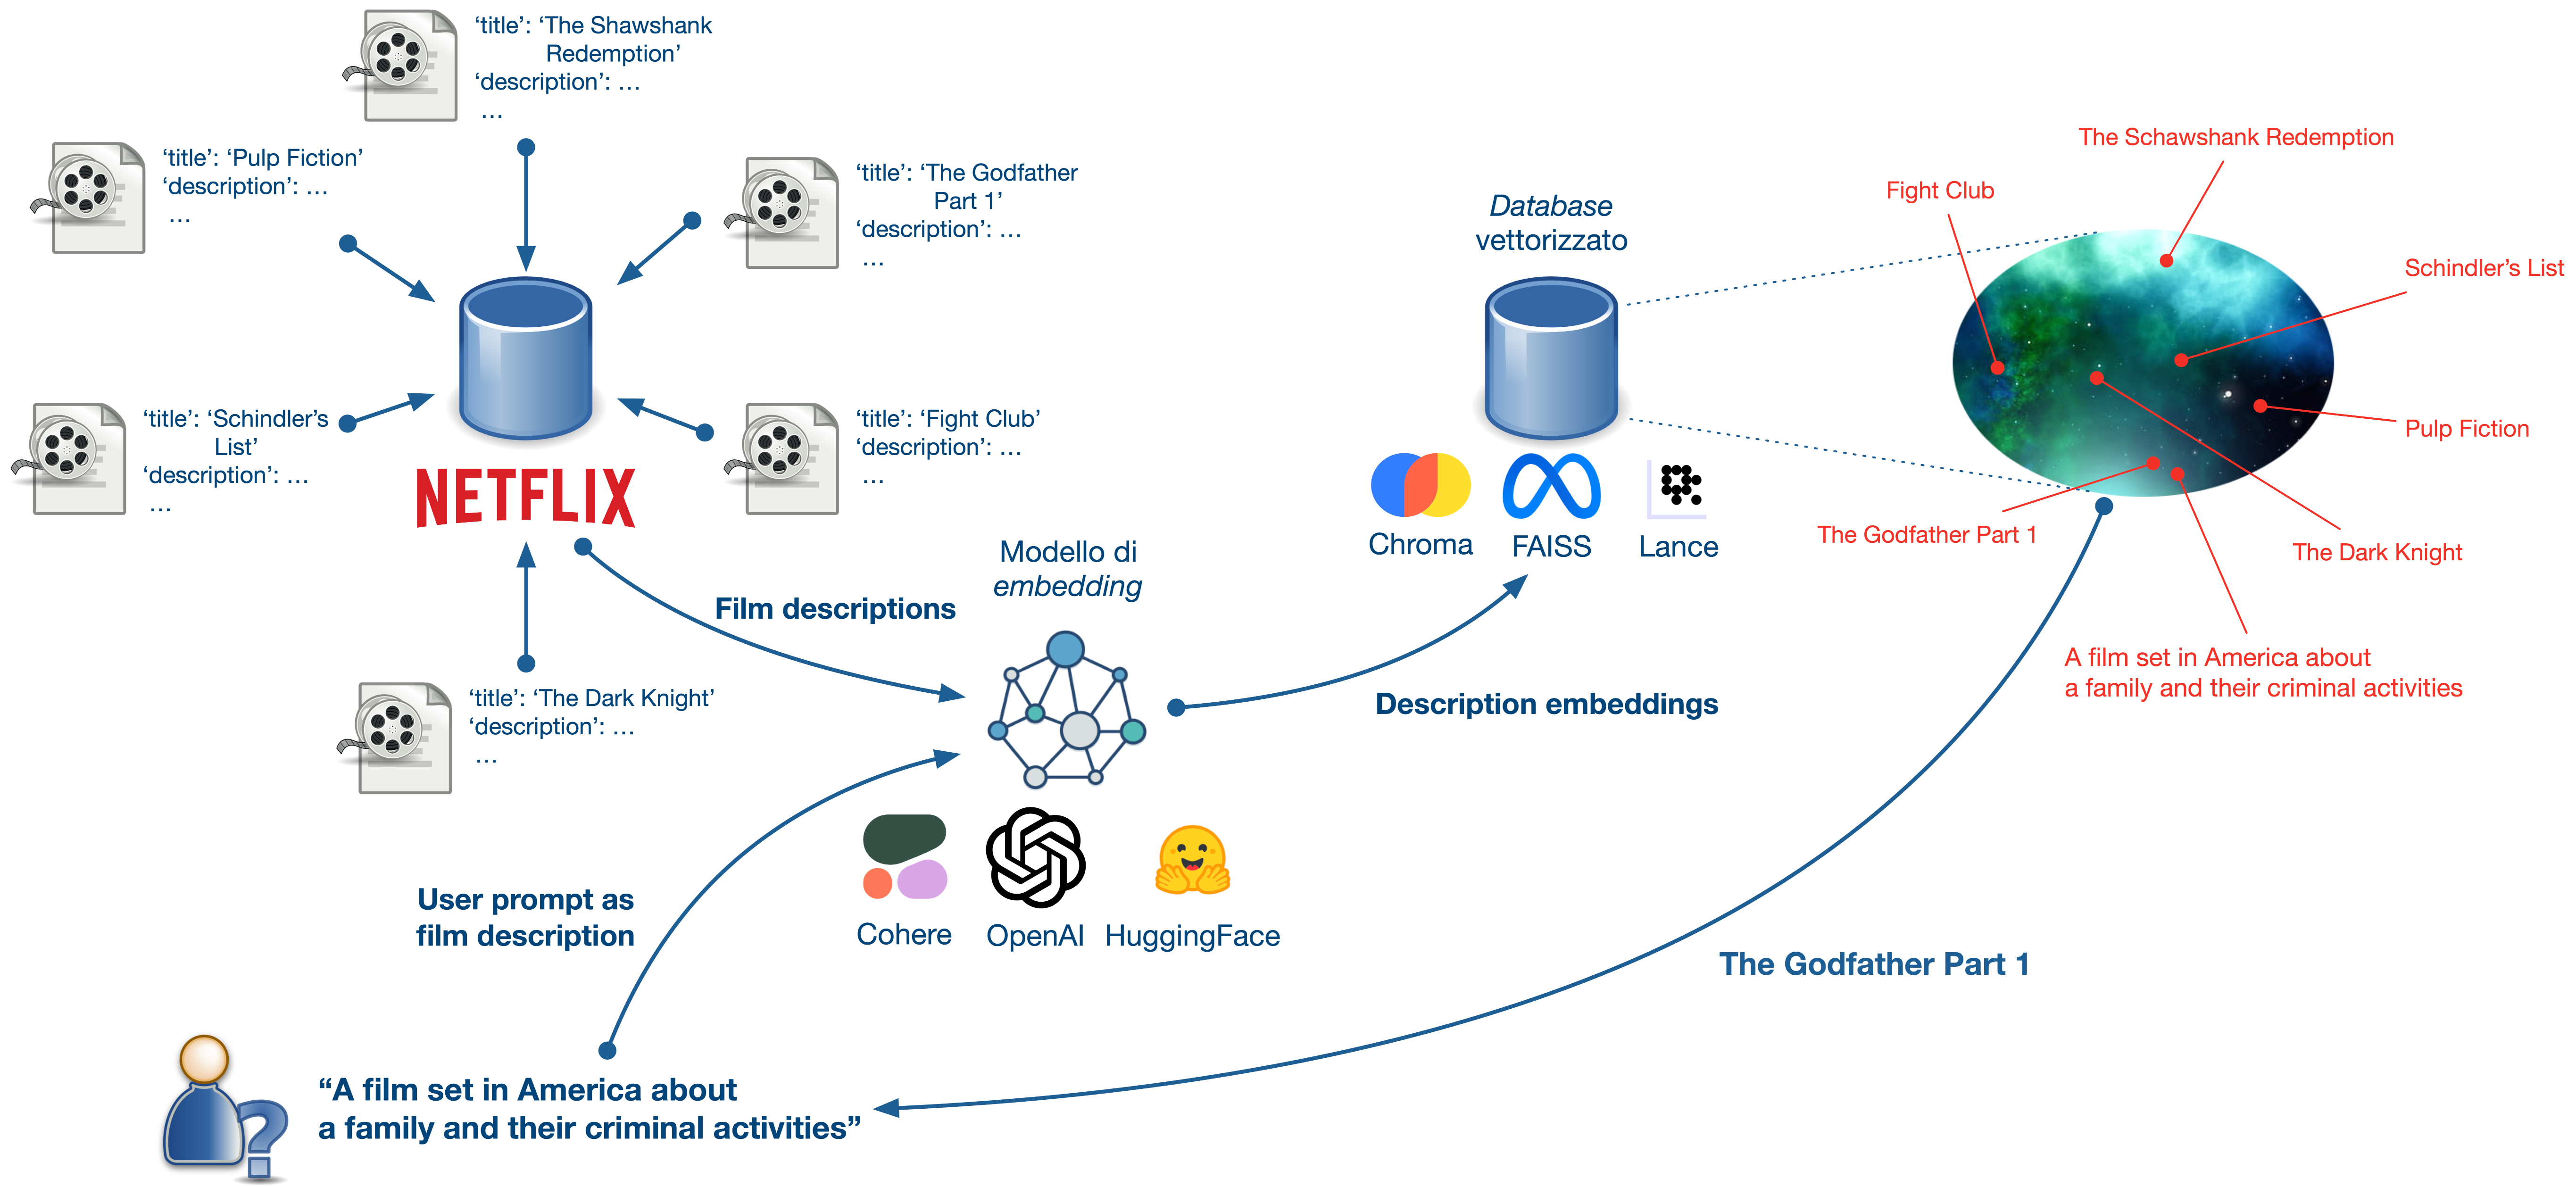
\includegraphics[width=\textwidth]{img/RAG-NO-LLM-NETFLIX-6-scaled.png}
    \end{center}
}
}
\end{frame}
%